%        File: prelimPres.tex
%     Created: Thu Aug 25 11:00 AM 2011 C
% Last Change: Thu Aug 25 11:00 AM 2011 C
%
%\documentclass[11pt,handout]{beamer}
\documentclass[9pt]{beamer}
\usetheme[white]{Wisconsin}
%\title[short title]{long title}
\title[Integrated Repository Model]{An Integrated Used Fuel Disposition and Generic Repository Model}
%\subtitle[short subtitle]{long subtitle}
\subtitle[Preliminary Report]{A Nuclear Engineering and Engineering Physics PhD Preliminary Report}
%\author[short name]{long name}
\author[K. Huff]{Kathryn D. Huff}
%\date[short date]{long date}
\date[9.01.2011]{September 1, 2011}
%\institution[short name]{long name}
\institute[UW-Madison]{University of Wisconsin-Madison}
% Page numbers.
\setbeamertemplate{footline}[page number]
% Those icons  in the references are terrible looking.
\setbeamertemplate{bibliography item}[text]
% need some error functions? Me too.
\DeclareMathOperator{\erf}{erf}
\DeclareMathOperator{\erfc}{erfc}


\begin{document}
%%%%%%%%%%%%%%%%%%%%%%%%%%%%%%%%%%%%%%%%%%%%%%%%%%%%%%%%%%%%%
%% From uw-beamer Here's a handy bit of code to place at 
%% the beginning of your presentation (after \begin{document}):
\newcommand*{\alphabet}{ABCDEFGHIJKLMNOPQRSTUVWXYZabcdefghijklmnopqrstuvwxyz}
\newlength{\highlightheight}
\newlength{\highlightdepth}
\newlength{\highlightmargin}
\setlength{\highlightmargin}{2pt}
\settoheight{\highlightheight}{\alphabet}
\settodepth{\highlightdepth}{\alphabet}
\addtolength{\highlightheight}{\highlightmargin}
\addtolength{\highlightdepth}{\highlightmargin}
\addtolength{\highlightheight}{\highlightdepth}
\newcommand*{\Highlight}{\rlap{\textcolor{HighlightBackground}{\rule[-\highlightdepth]{\linewidth}{\highlightheight}}}}
%%%%%%%%%%%%%%%%%%%%%%%%%%%%%%%%%%%%%%%%%%%%%%%%%%%%%%%%%%%%%

%||||||||||||||||||||||||||
\AtBeginSection[]
{
   \begin{frame}
       \frametitle{Outline}
       \tableofcontents[currentsection]
   \end{frame}
}

%||||---------------
\frame{
\titlepage
}
%---------------||||


%||||---------------
\frame{
\frametitle{Outline}
\tableofcontents[]
}
%---------------||||
\section{Introduction}
\subsection{Motivation}
% Waste is a problem
% Decisionmakers are contemplating many fuel cycle options
% Decisionmakers are contemplating many repository options
% Interfacing between FCO/SA campaign and UFD campaign

\begin{frame}[ctb!]
  \frametitle{Future Disposal System Options}
   \begin{minipage}{0.44\textwidth}
     \begin{figure}[h!]
         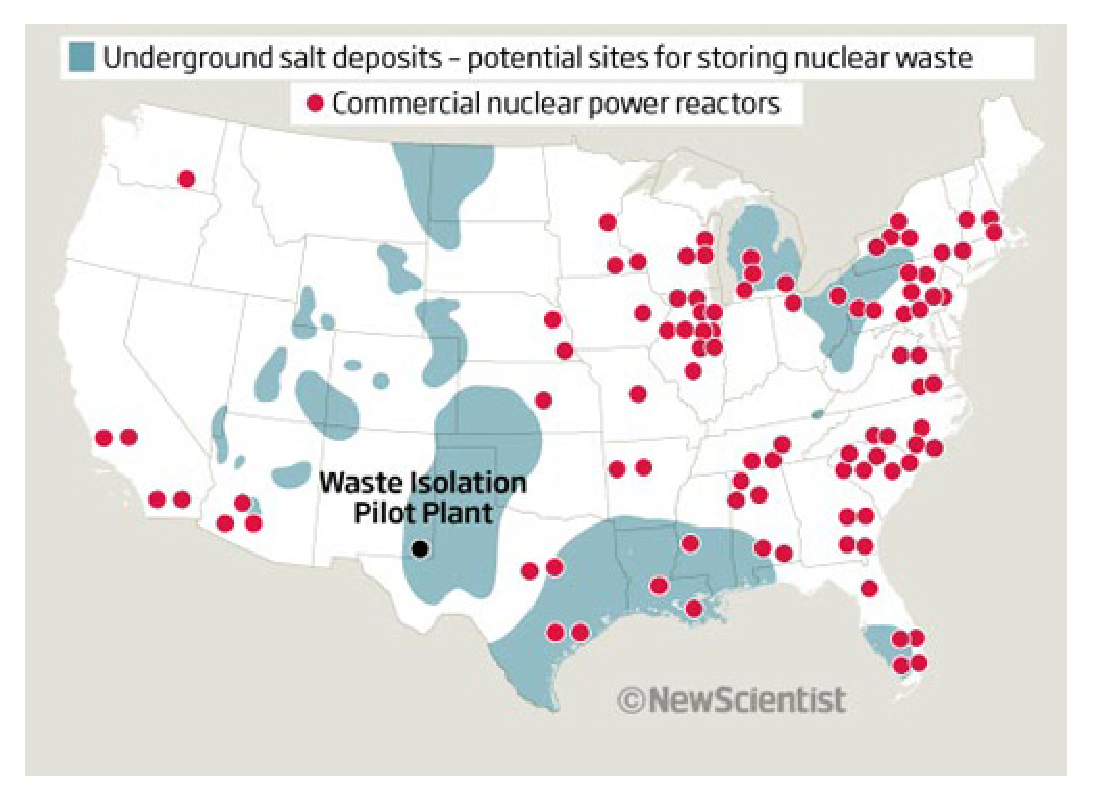
\includegraphics[width=0.8\textwidth]{saltNewScientist.eps}
         \caption{U.S. Salt Deposits ref. \cite{newscientist_where_2011}}
     \end{figure}
     \begin{figure}[h!]
         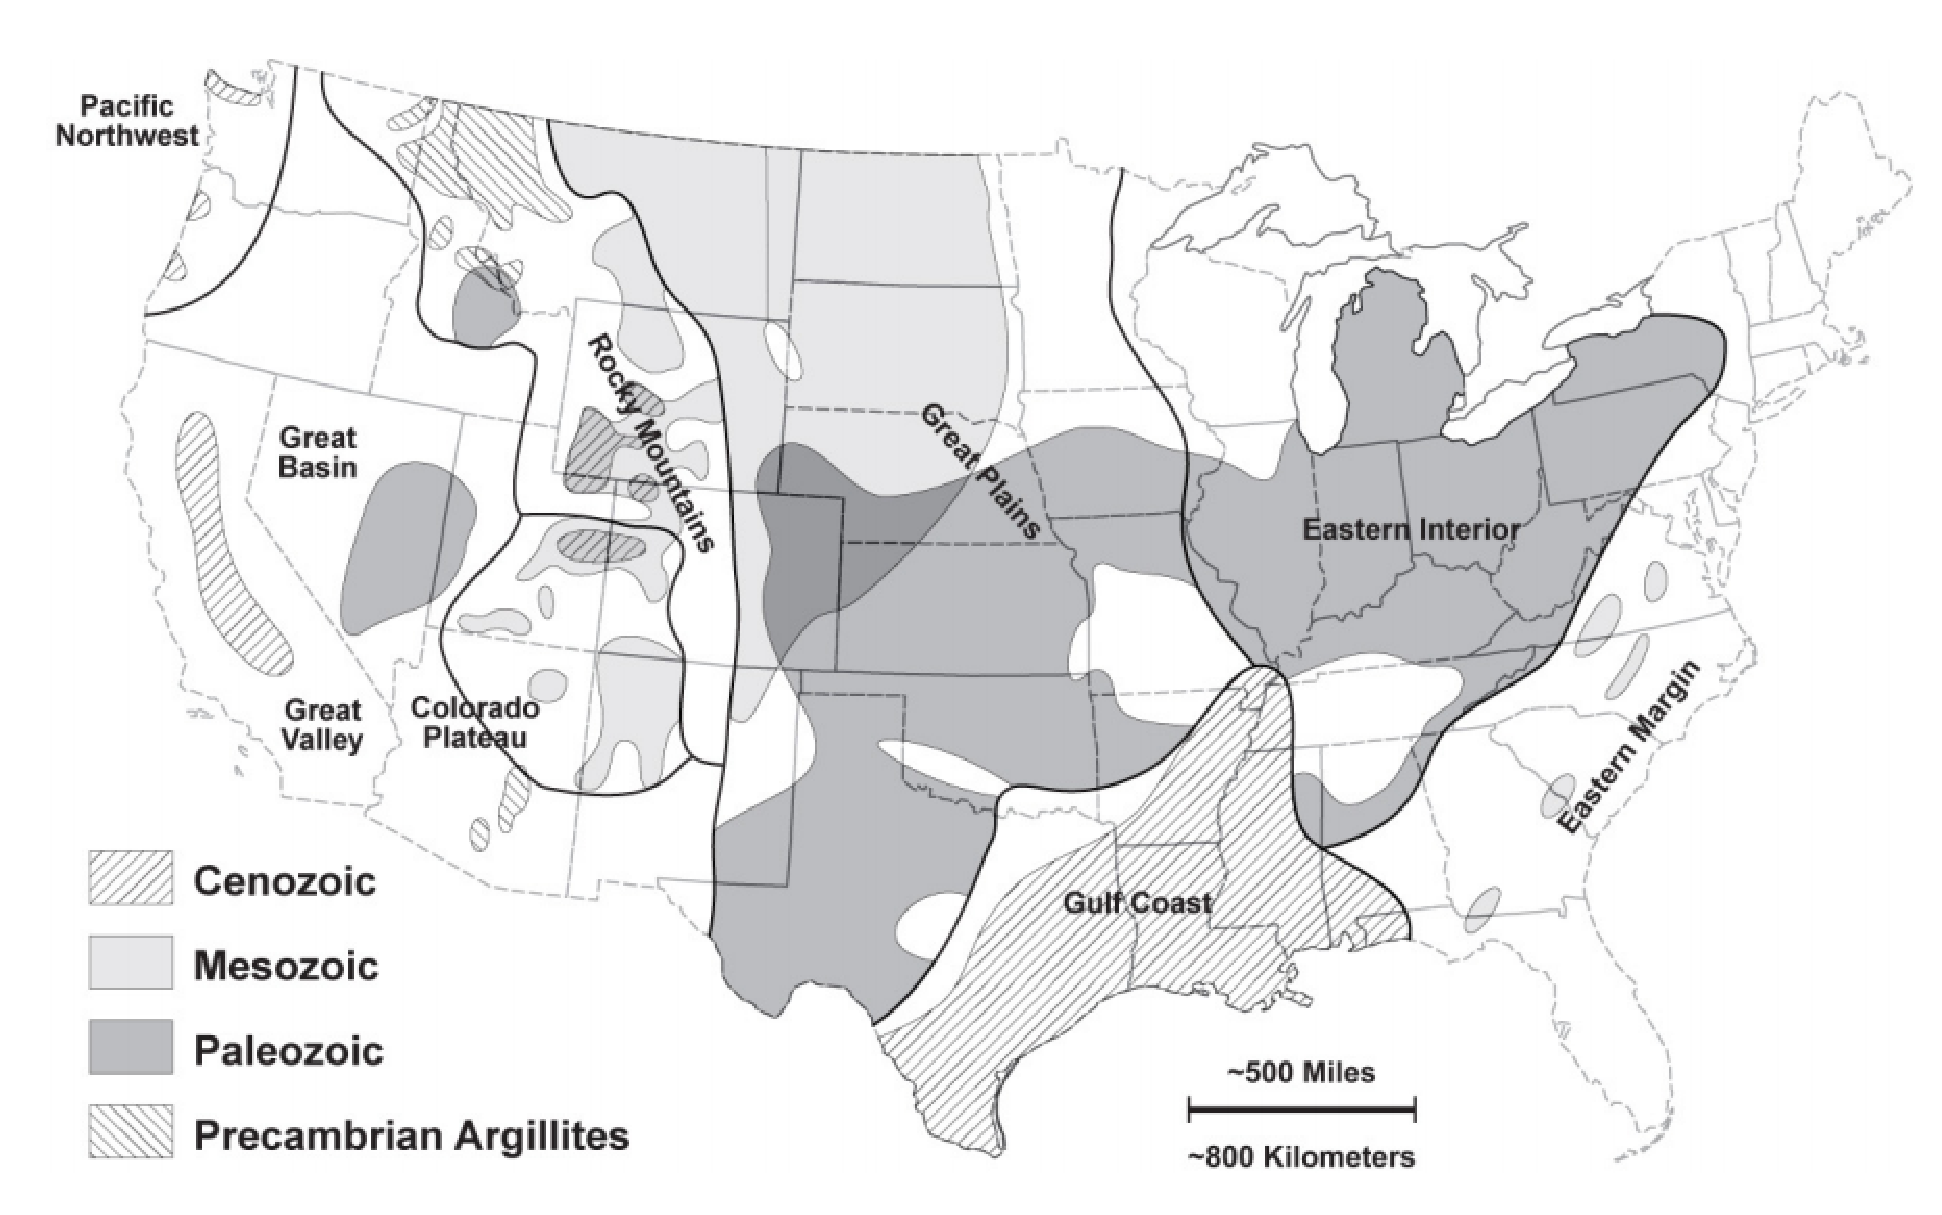
\includegraphics[width=0.8\textwidth]{clayGonzales.eps}
         \caption{U.S. Clay Deposits ref. \cite{gonzales_shales_1985}}
     \end{figure}
   \end{minipage}
   \hspace{0.01cm}
   \begin{minipage}{0.44\textwidth}
     \begin{figure}[h!]
         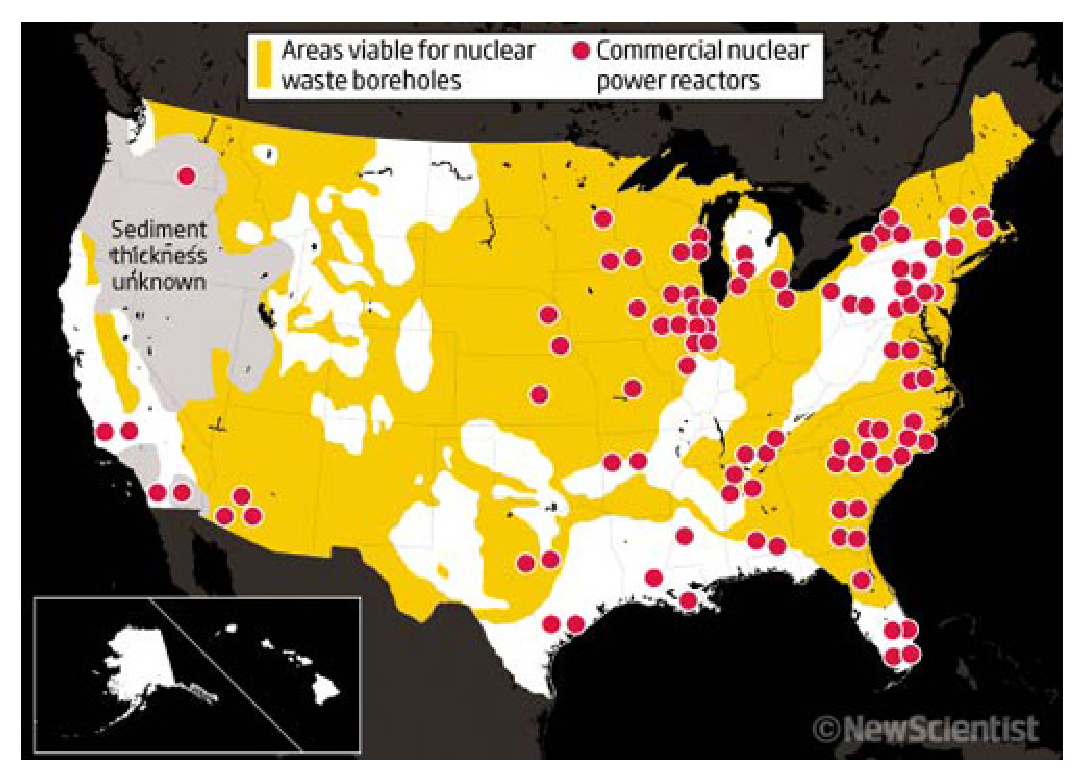
\includegraphics[width=0.8\textwidth]{boreholeNewScientist.eps}
         \caption{U.S. Crystalline Basement ref.  \cite{newscientist_where_2011}}
     \end{figure}
     \begin{figure}[h!]
         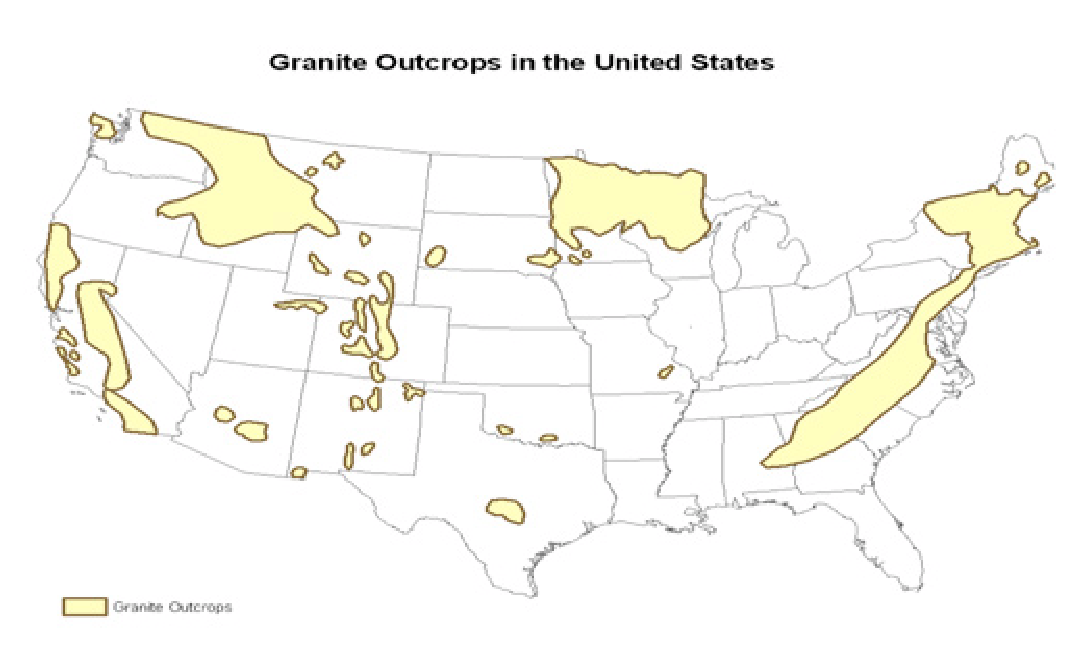
\includegraphics[width=0.8\textwidth]{graniteBush.eps}
         \caption{U.S. Granite ref. \cite{bush_economic_1976}}
     \end{figure}
   \end{minipage}
\end{frame}


\begin{frame}[ctb!]
  \frametitle{Future Fuel Cycle Options}
   % Future Fuel Cycles
    \begin{table}
      \centering
      \footnotesize{
      \begin{tabular}{|l|l|l|}
        \multicolumn{3}{c}{\textbf{Domestic Fuel Cycle Options}}\\
        \hline
        Title & Description& Challenges \\
        \hline
        Open          & Once Through         & High Temperatures, Volumes \\
                      & Current US PWR Fleet &      \\
                      & No Separations       &      \\
                      & No Recycling         &      \\
                      & Higher Burnups &      \\
        Modified Open & Partial Recycling    & Both high volumes and myriad fuel streams \\
                      & Next Gen. PWR Fleet &      \\
                      & Limited Separations  &      \\
                      & Limited Transmutation &      \\
                      & Advanced Fuel Forms  &      \\
        Closed        & Full Recycling       & Myriad fuel streams \\
                      & Full Separations &      \\
                      & Full Recycling &      \\
                      & VHTGR, SFRs, &      \\
                      & <++> &      \\
                      & <++> &      \\
                      & <++> &      \\
                      & <++> &      \\
                      & <++> &      \\
        \hline
      \end{tabular}
      \caption[Fuel Cycle Options]{Domestic Fuel Cycle Options }
      \label{tab:fco}
      }
    \end{table}
\end{frame}



\subsection{Methodology}
% Overview : 
% put a repository model into cyclus
% that is capable of distinguishing between disposal choices
% and fuel cycle choices
% but is still speedy. 

\begin{frame}[ctb!]
  \frametitle{Methodology : Modularity }
  A modular repository framework facilitates 
  \begin{itemize}
    \item  interchangable subcomponents (e.g. buffer material) so that 
      the impact on the disposal system performance may be observed
    \item and simulations with varying levels of detail.
  \end{itemize}
 \pause
  Integration with a fuel cycle simulator facilitates
  \begin{itemize}
    \item analysis of feedback effects upon the fuel cycle
    \item and investigation of fuel cycle choices on disposal system 
      performance.
  \end{itemize}
\end{frame}

\begin{frame}[ctb!]
  \frametitle{Methodology : Abstraction for Efficiency}

  \begin{minipage}{0.49\textwidth}
      Abstraction simplifies models while capturing salient physics. 
      Parametric analysis with detailed models will inform simpler models at the 
      level of detail important for fuel cycle analysis.
    \begin{figure}[h!]
        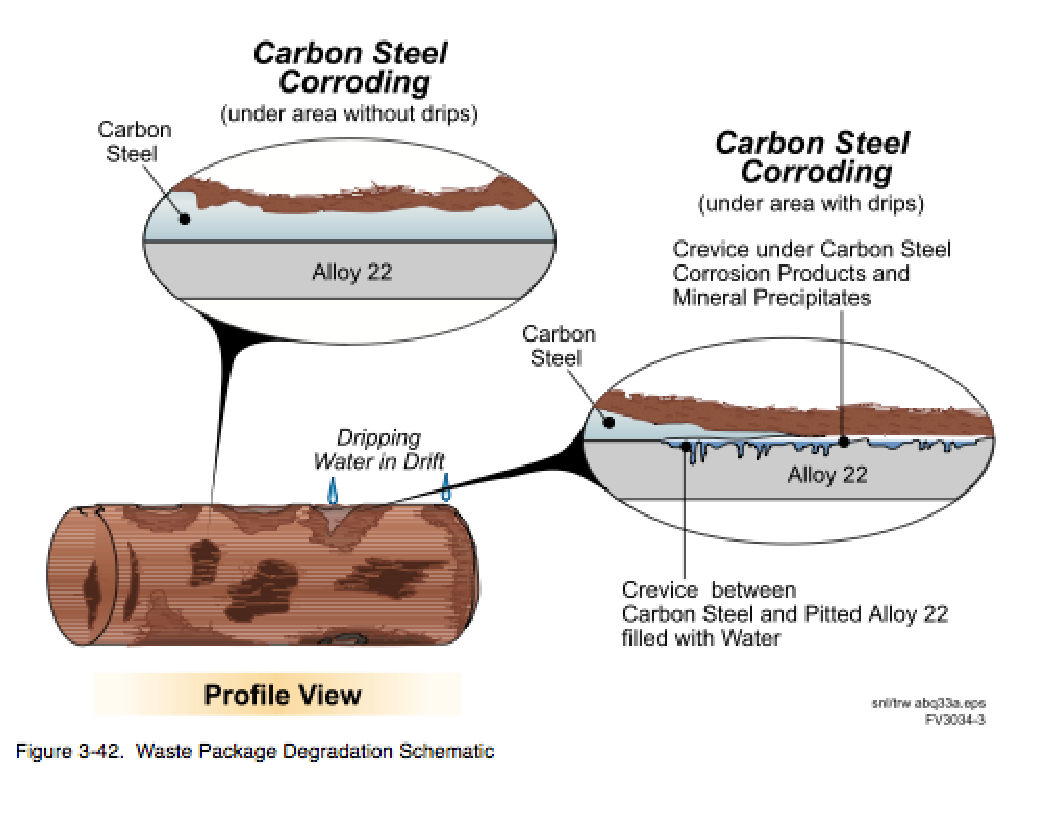
\includegraphics[width=\textwidth]{reality.eps}
      \caption{A complex computational model is an abstraction of reality 
      \cite{doe_viability_1998}.}
      \label{fig:reality}
    \end{figure}
  \end{minipage}
  \hspace{0.01cm}
  \begin{minipage}{0.49\textwidth}
    \begin{figure}[h!]
        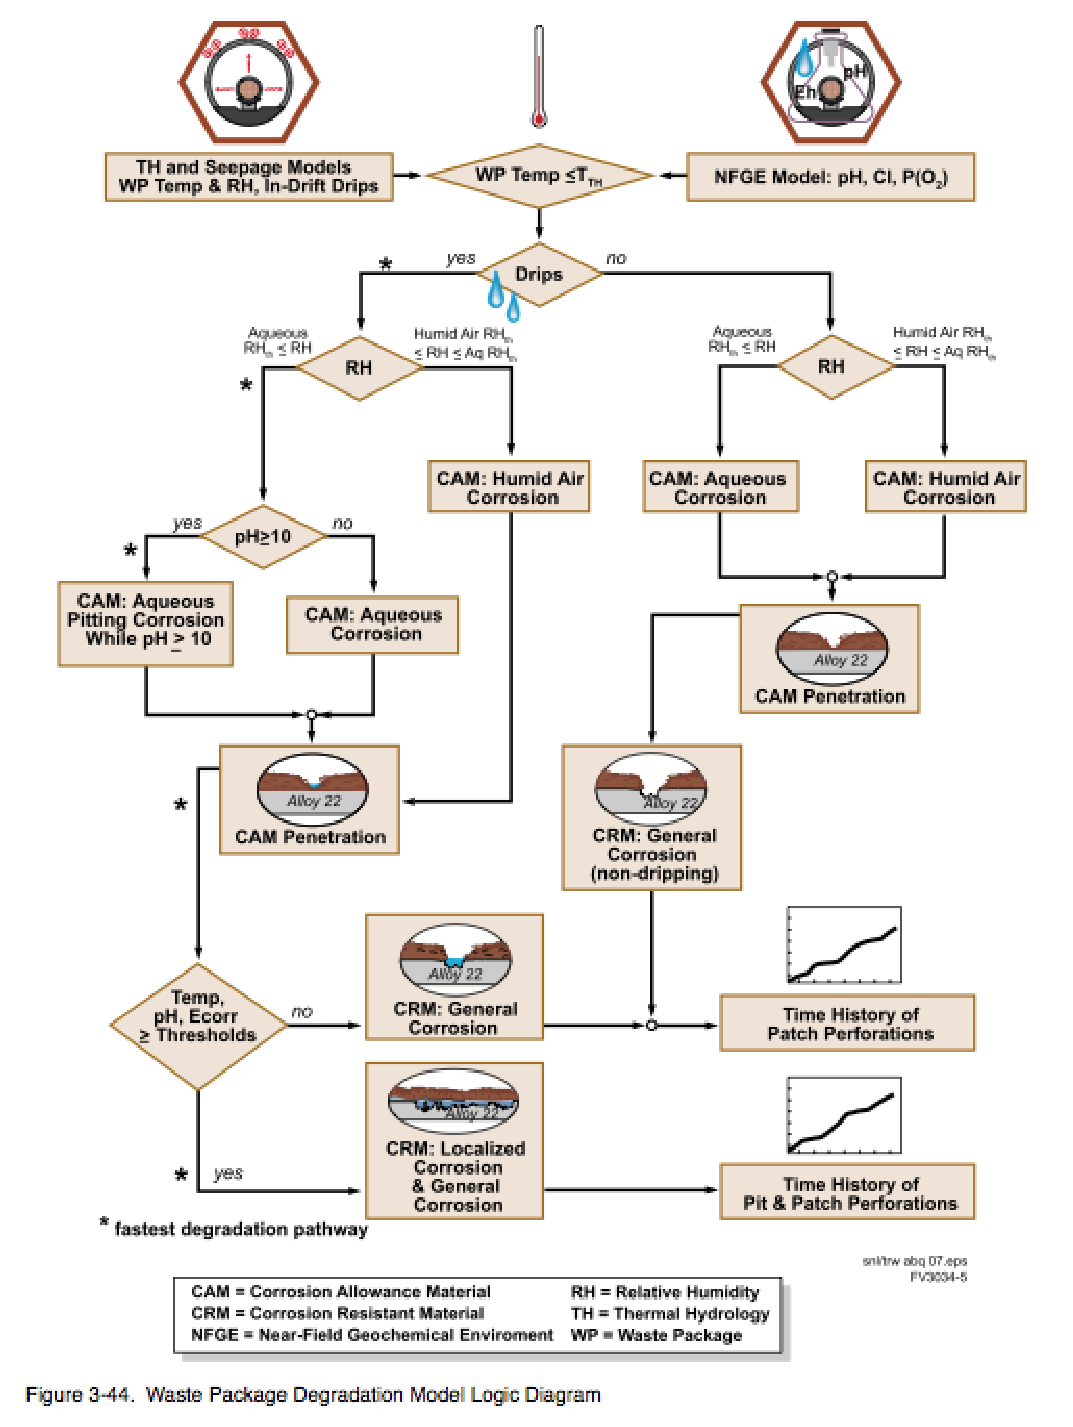
\includegraphics[width=0.9\textwidth]{model.eps}
    \end{figure}
  \end{minipage}
  

\end{frame}

\section{Literature Review}
\subsection{Repository Capabilities within Systems Analysis Tools}

% They just report mass flows
% or are proprietary and super long running

\begin{frame}[ctb!]
  \frametitle{Top Level Fuel Cycle Simulators}
  % most only report mass flows.
  \begin{figure}[htbp!]
    \begin{center}
      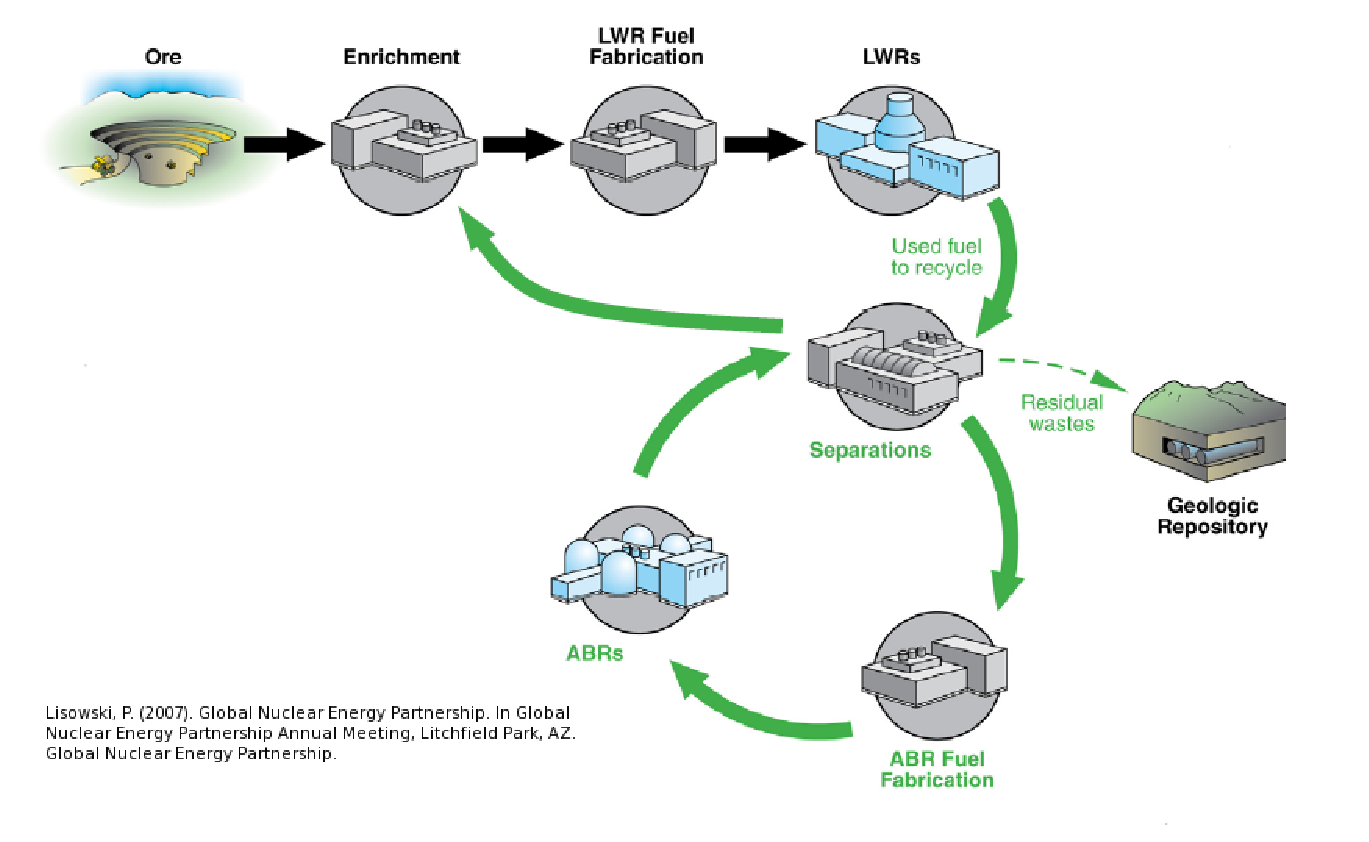
\includegraphics[height=4cm]{./images/simulations.eps}
    \end{center}
    \caption{Top level simulators are intended to model the collective 
    behavior of various fuel cycle decisions and 
    strategies \cite{lisowski_global_2007}.}
    \label{fig:simulation}
  \end{figure}
\end{frame}

\begin{frame}[ctb!]
  \frametitle{Need For an Integrated Repository Model}
  % Incorporates disposal system decisions into metrics information
  % Captures Feedbacks
  Current fuel cycle simulators neglect disposal system decisions and 
  repository behavior. Most report masses and mass indexed metrics such 
  as radiotoxicity, both meaningless without release pathway analysis
  and not informative for disposal system options.

  %        File: systools_tab.tex
%     Created: Mon Aug 29 09:00 AM 2011 C
% Last Change: Mon Aug 29 09:00 AM 2011 C
%
\begin{table}
  \centering
  \footnotesize{
  \begin{tabular}{|l|l|c|c|c|}
    \multicolumn{5}{c}{\textbf{Repository Capabilities within Systems Analysis Tools}}\\
    \hline
    Tool & Institution & Fuel Disposition & Radionuclide Transport & Heat Transport  \\
    \hline
    NUWASTE\cite{abkowitz_nuclear_2010} & NWTRB & yes & no & no \\
    VISION \cite{yacout_vision_2006} & INL   & yes & no & YMR only \\
    DANESS \cite{van_den_durpel_daness:_2006} & ANL   & no & no & no \\
    COSI   \cite{boucher_international_2010} & CEA   & yes & no & yes \\
    NFCSim \cite{schneider_nfcsim_2004} & LANL  & no & no & no \\
    CAFCA  \cite{guerin_benchmark_2009} & MIT   & no & no & no \\
    ORION  \cite{guerin_benchmark_2009} & BNL   & no & no & no \\
    TSM    \cite{turner_discrete_2010} & OCRWM & yes & no & YMR only \\
    \hline
  \end{tabular}
  \caption[System Tools]{System tools are lacking in radionuclide transport and  
  heat transport calculations in generic geologic media.}
  \label{tab:systools}
  }
\end{table}




\end{frame}


\subsection{Conceptual Discussion of Disposal Environments}
% layouts
% EBS choices
% Geologies


\begin{frame}[ctb!]
  \frametitle{Clay Disposal Environments}

  \begin{figure}[h!]
    \begin{center}
      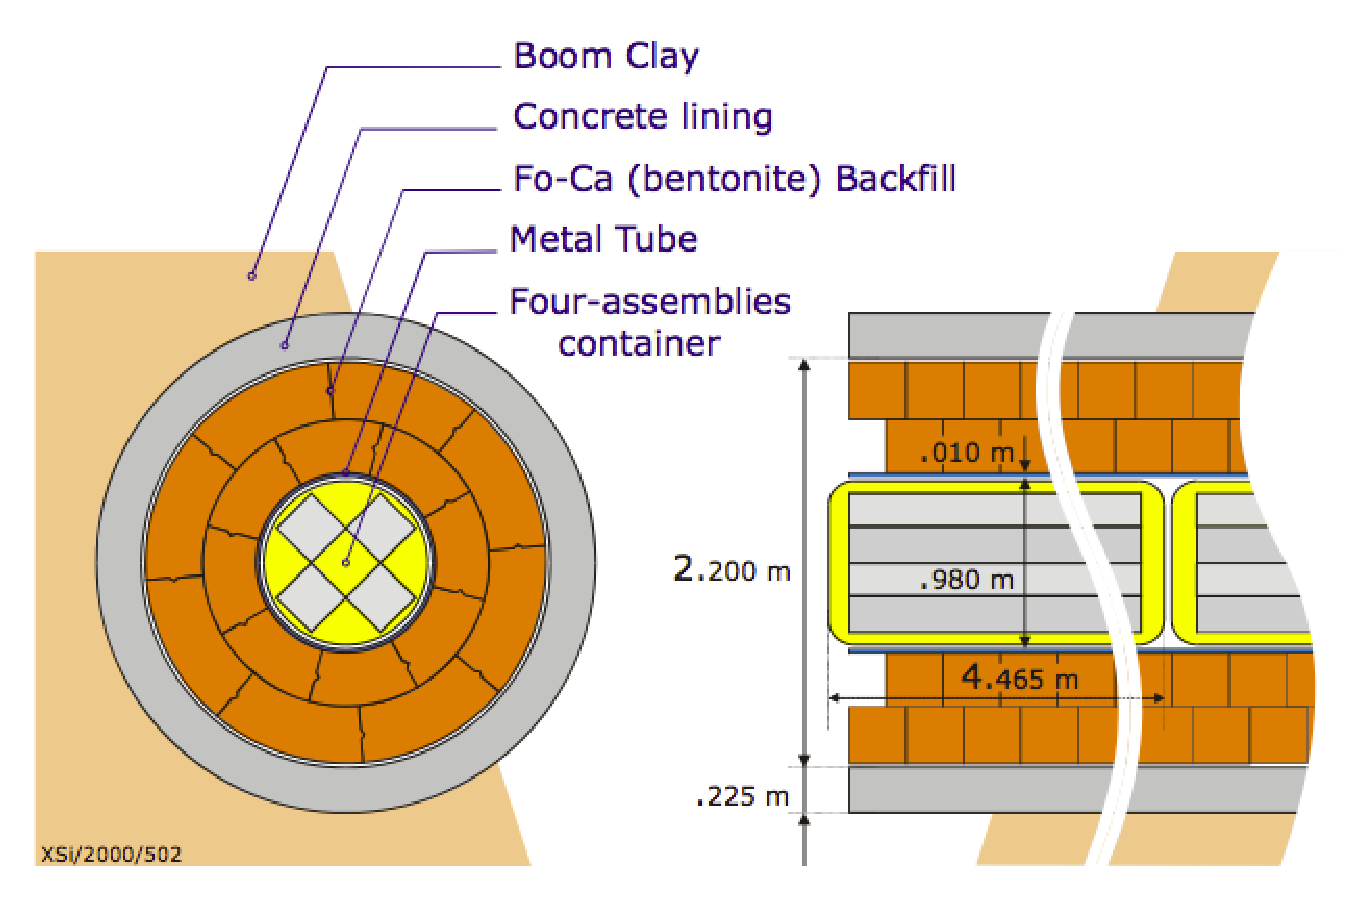
\includegraphics[height=.7\textheight]{belgianClayRedImp.eps}
    \end{center}
    \caption{Belgian reference concept in Boom Clay 
    \cite{von_lensa_red-impact_2005}.}
    \label{fig:belgianClayRedImp}
  \end{figure}

\end{frame}

\begin{frame}[ctb!]
  \frametitle{Granite Disposal Environments}

  \begin{figure}[h!]
    \begin{center}
      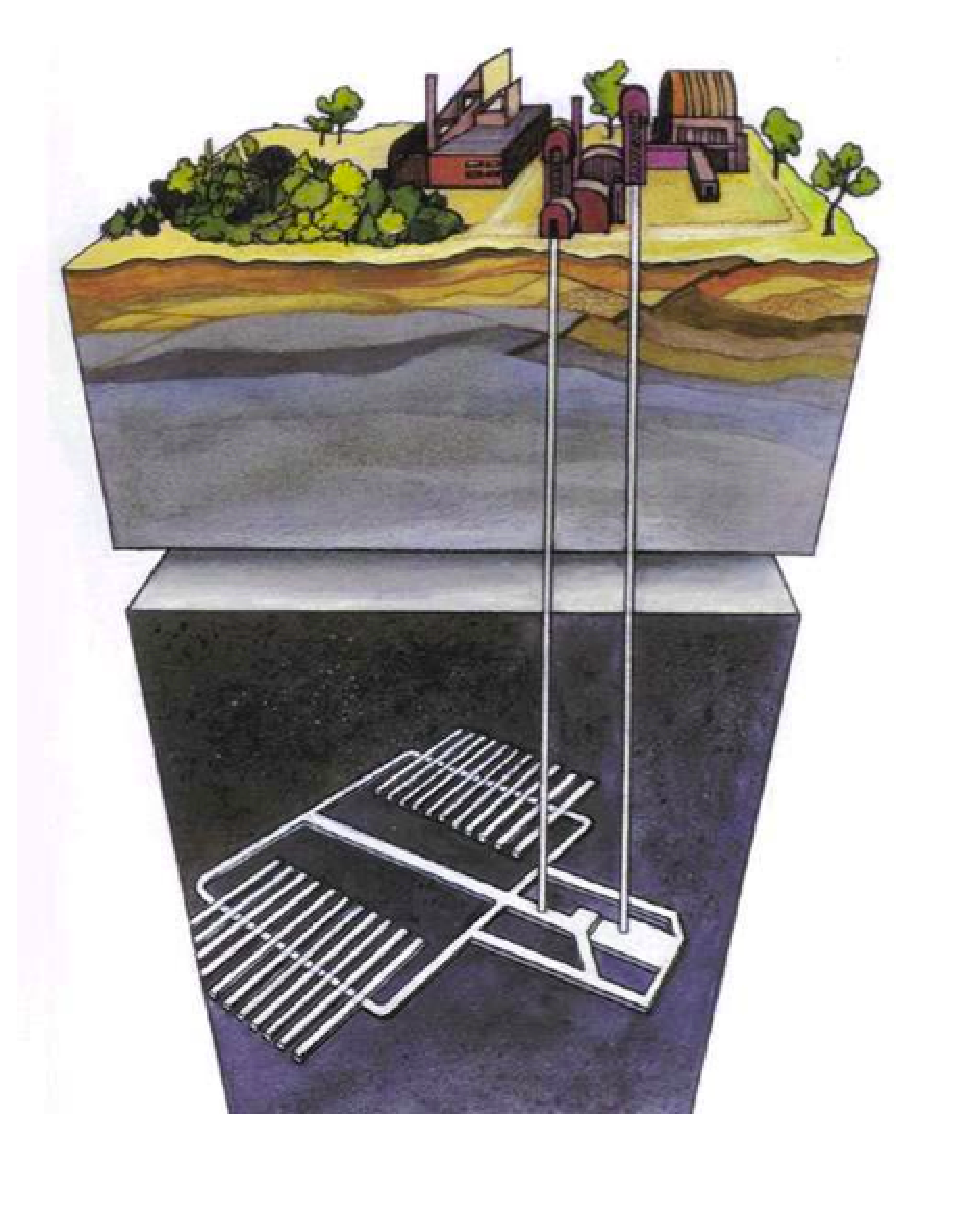
\includegraphics[height=.7\textheight]{czechGraniteRedImp.eps}
    \end{center}
    \caption{Czech reference concept in Granite 
    \cite{von_lensa_red-impact_2005}.}
    \label{fig:czechGraniteRedImp}
  \end{figure}

\end{frame}

\begin{frame}[ctb!]
  \frametitle{Salt Disposal Environments}

  \begin{figure}[h!]
    \begin{center}
      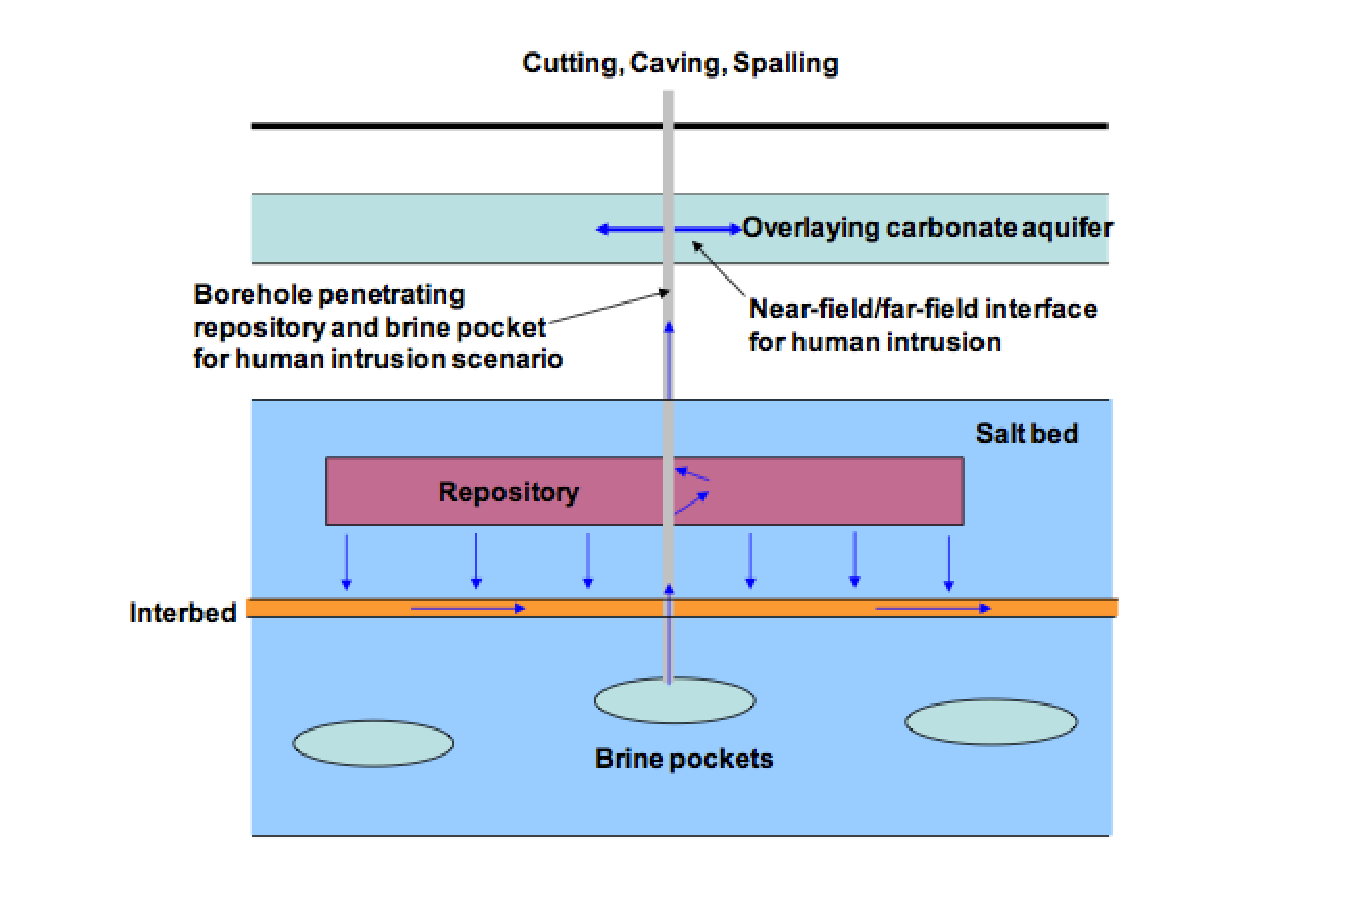
\includegraphics[height=.7\textheight]{saltGPAM.eps}
    \end{center}
    \caption{DOE-NE Used Fuel Disposition Campaign  concept in 
    Salt \cite{clayton_generic_2010}.}
    \label{fig:saltGPAM}
  \end{figure}

\end{frame}

\begin{frame}[ctb!]
  \frametitle{Deep Borehole Disposal Environment}

  \begin{figure}[h!]
    \begin{center}
      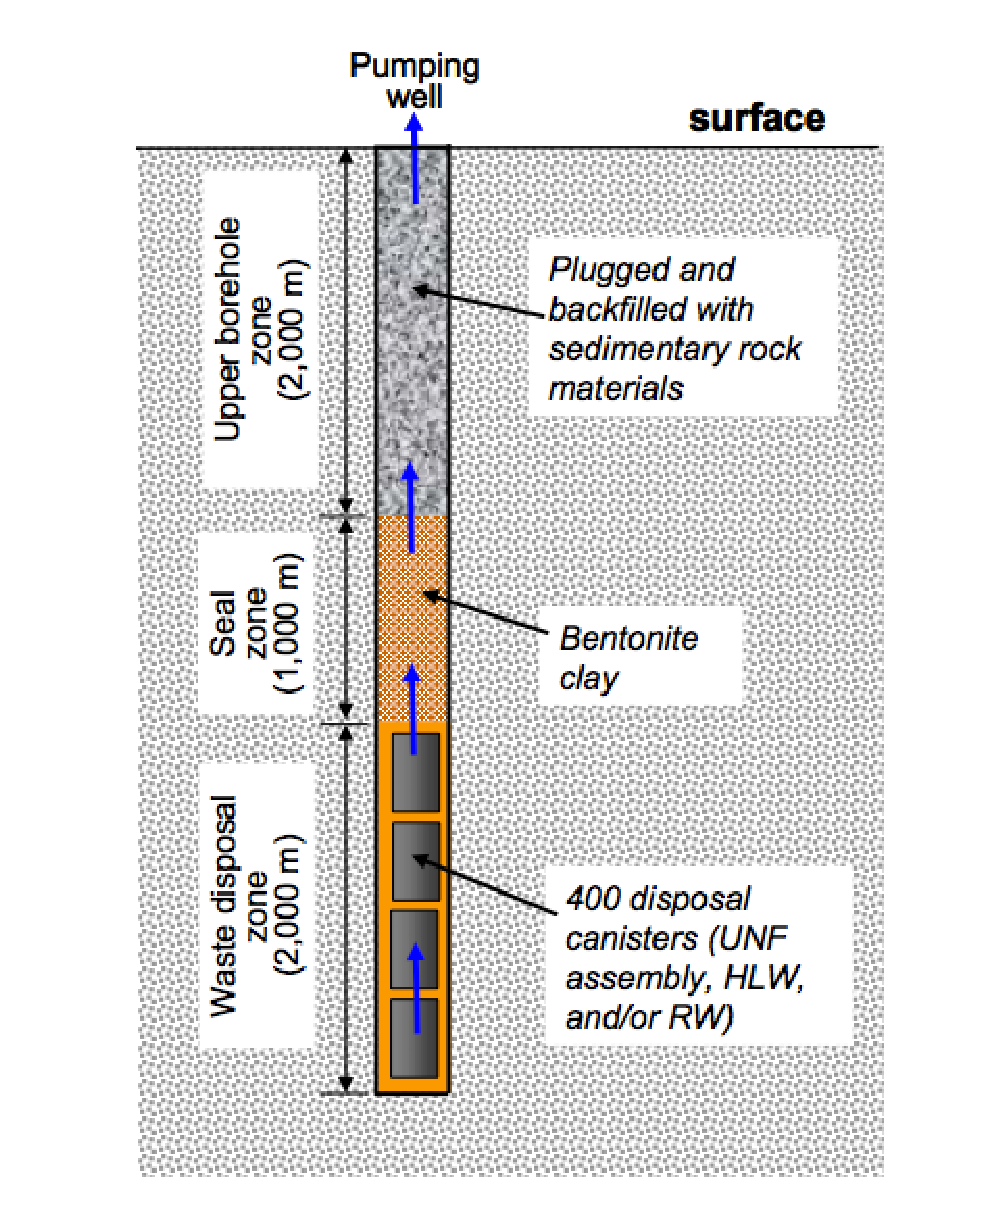
\includegraphics[height=.7\textheight]{boreholeGPAM.eps}
    \end{center}
    \caption{DOE-NE Used Fuel Disposition Campaign Deep Borehole concept 
    \cite{clayton_generic_2010}.}
    \label{fig:boreholeGPAM}
  \end{figure}

\end{frame}


\begin{frame}
  \frametitle{Repository Layouts}

  \begin{minipage}{0.49\textwidth}
    \begin{figure}[h!]
      \includegraphics[width=0.75\textwidth]{boreholes.eps}
    \end{figure}
    \begin{figure}[h!]
      \includegraphics[width=0.75\textwidth]{vertical.eps}
    \end{figure}
  \end{minipage}
  \hspace{0.01cm}
  \begin{minipage}{0.49\textwidth}
    \begin{figure}[h!]
      \includegraphics[width=0.8\textwidth]{horizontal.eps}
    \end{figure}
    \begin{figure}[h!]
      \includegraphics[width=0.8\textwidth]{alcoves.eps}
    \end{figure}
  \end{minipage}

\end{frame}

\begin{frame}[ctb!]
  \frametitle{All Disposal Environments}
  % Table
  %        File: geos_tab.tex
%     Created: Thu Aug 04 11:00 AM 2011 C
% Last Change: Thu Aug 04 11:00 AM 2011 C
%
\begin{table}[h!]
  \centering
  \footnotesize{
  \begin{tabular}{|l|r|r|r|r|}
    \multicolumn{5}{c}{\textbf{Features of Various Concepts}}\\
    \hline
    Feature & Clay & Granite & Salt & Deep Borehole \\ 
    \hline
    \multicolumn{5}{|c|}{\textbf{Hydrology}}\\
    \hline
    Total Porosity $[\%]$    & 34-60  & 0.1 & 0.5 & 0-0.5 \\ 
    Eff. Porosity $[\%]$ & 0.5-5 & 0.0005 & 0.1 & 0.00005-0.01 \\ 
    Conductivity$[m/s]$ & $10^{-11} - 10^{-9}$ & 
    $10^{-6}-10^{-5}$ & $10^{-12}-10^{-10}$ & 
    $10^{-13}-10^{-4}$ \\ 
    Fracturation & none & high & none & low at depth \\ 
    \hline
    \hline
    \multicolumn{5}{|c|}{\textbf{Geochemistry}}\\
    \hline
    Reducing & Near \& Far Field & NF only  & NF only & NF only \\
    Oxidizing & none & Slight in FF & Slight in FF & Slight in FF \\
    Salinity & higher at depth & higher at depth & high & high \\
    pH & $\sim7$ & $\ge7$ & $\ge7$ & $\sim7$ \\
    \hline
    \hline
    \multicolumn{5}{|c|}{\textbf{Design}}\\
    \hline
    Waste Package & Steel, Cu & Steel, Cu & Steel & Steel,Cement \\
    Buffer & -,Fo-Ca,Cement & Fo-Ca,Cement & Crushed Salt & -,Fo-Ca,Cement\\ 
    Depth & 100-500 m & 100-500 m & 100-500m & 3-5km \\ 
    Emplacement & Vert.,Horiz,Alcove & Vert.,Horiz. & Alcove & Vert. \\ 
    Packages/Gallery & one, many & one, many & one, two & 400 \\ 
    \hline
    \hline
    \multicolumn{5}{|c|}{\textbf{Thermal Behavior}}\\
    \hline
    Buffer Limit $[^{\circ}C]$ & 100 (Fo-Ca) & 100 (Fo-Ca) & 180 & 100 (Fo-Ca) \\ 
    Host Limit $[^{\circ}C]$   & 100 (alteration)  & 200 (cracking) & 180 (brines) & none \\ 
    Conductivity $[\frac{W}{m{\cdot}K}]$ & $1-2$ & $2-4$ & $\sim4$  & $2-4$ \\ 
    Coalesence & yes & no & yes & no \\ 
    \hline
  \end{tabular}
  }
  \label{tab:geos_tab}
\end{table}
%  \cite{stober_hydraulic_2006} 

\end{frame}


\subsection{Models of Radionuclide Transport}


\begin{frame}[ctb!]
  \frametitle{Radionuclide Transport}
  % Map the path out of the repository.
  % WP failure, WF dissolution, 
  \begin{minipage}{0.49\textwidth}
  \begin{figure}[h!]
      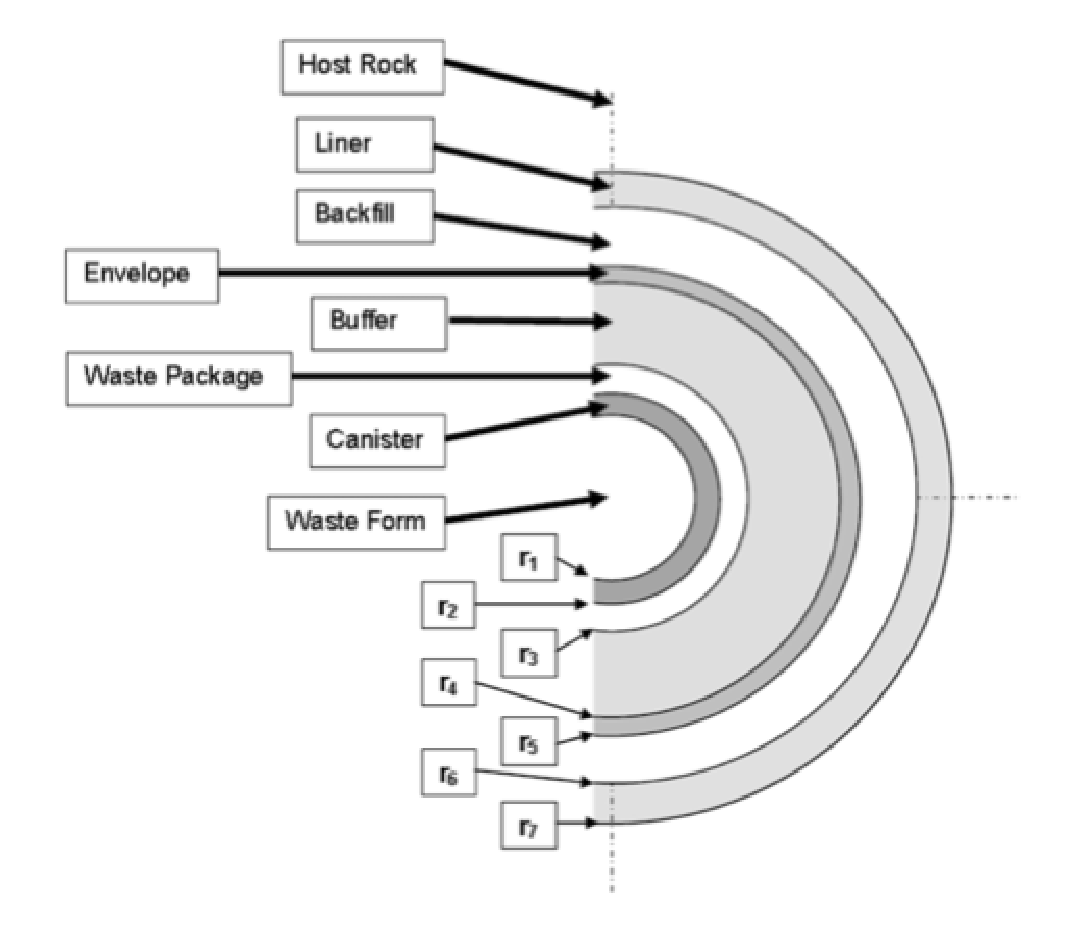
\includegraphics[width=\textwidth]{ebsLayersLLNL.eps}
    \caption{After waste package failure, radionuclides pass through successive 
    layers of the engineered barrier system \cite{greenberg_thermal_2011}.}
    \label{fig:ebsLayersLLNL}
  \end{figure}
  \end{minipage}
  \hspace{0.01cm}
  \begin{minipage}{0.49\textwidth}
    \begin{itemize}
      \item Source Term - Radionuclide mass flux to the environment
        \begin{itemize}
          \item Safety and Risk Metric
          \item EPA Regulation
        \end{itemize}
      \item Radionuclide transport is a function of
        \begin{itemize}
          \item Geochemistry - chemically induced material degradation, 
            radionuclide solubility limits, sorption, colloid mobility, etc.
          \item Hydrology - water induced material degradation, 
            water movement through pores and fractures, 
            dissolved contaminant dispersion. 
          \item Thermal Effects - thermally induced material degradation, 
            thermal hydrological effects.
        \end{itemize}
    \end{itemize}
  \end{minipage}
\end{frame}


\begin{frame}[ctb!]
  \frametitle{Waste Form Release Models}
  % Waste forms
  \footnotesize{%        File: litrev/wf_tab.tex
%     Created: Fri Aug 05 09:00 AM 2011 C
% Last Change: Fri Aug 05 09:00 AM 2011 C
%
\begin{table}[h!]
  \centering
  \footnotesize{
  \begin{tabular}{|l|l|c|c|}
    \multicolumn{4}{c}{\textbf{Waste Form Types}}\\
    \hline
    WF Type & SubTypes & Contents & Release Drivers  \\
    \hline
    \hline
    Once         & CSNF Ceramic Oxide & Nominal BU UOx \& MOX & redox rxns \\
     Through     & CSNF Ceramic Oxide & High BU UOx \& MOX & redox rxns, heat  \\
                 & HTGR TRISO Graphite & High BU & graphite rxns\\
                 & DSNF Metal  & High BU N Reactor Fuel & metal rxns,  heat\\
                 & DSNF Carbides  & Fast Reactor Fuels & carbide rxns,  heat\\
                 & DSNF Ceramic Oxides  & Research Reactor Fuels & redox rxns,  heat\\
    \hline
    Borosilicate & Current & MA, Cs/Sr & heat, alteration \\
     Glass       & Future & Mo, no MA no Cs/Sr & alteration  \\
    \hline
    Glass & Glass Bonded Sodalite & Echem treated UOx, MOX & redox, alteration\\
    Ceramic  &&&\\
    \hline
    Metal & From Echem & Cladding, noble metals & metal rxns, heat \\
    Alloy       & From Aqueous & transition metals & metal rxns, heat  \\
    \hline
    Advanced &  & volatized iodine  & ceramic rxns, redox \\
    Ceramic &&&\\
    \hline
    Salt  & Cementitious Sodium  & separated streams  & alkaline rxns, dissolution \\
    \hline
  \end{tabular}
  \caption[Waste Form Types]{An array of waste forms developed for nuclear 
  wastes will have a corresponding array of dominant release mechanisms \cite{blink_disposal_2010}}.
  \label{tab:wf}
  }
\end{table}


}
\end{frame}


\begin{frame}[ctb!]
  \frametitle{Waste Package Failure Models}
  % Waste Package
   
    \footnotesize{
    Waste package failure can, in general, be represented with an expression of the 
    number of failed waste packages, $n_F$ failing per unit time. This is a simple 
    product between the initial number of waste packages, $N$, and the rate, $f$, of 
    failure,
    \begin{align}
      n_F = N\cdot f().
      \intertext{This rate may be a physical function,}
      f() = N\cdot f(t,T,\cdots),
      \intertext{or any time dependent function,}
      f()=f(t),
      \intertext{of which instantaneous failure is a special case,}
      f()= \delta(t-t_F),
      \intertext{as is the Weibull distribution,}
      f(t,\lambda,k) =  \begin{cases}
        \frac{k}{\lambda}\left(\frac{t}{\lambda}\right)^{k-1}e^{-(t/\lambda)^{k}} & 
        t\geq0 ,\\
        0 & t<0 .\end{cases}
    \end{align}
    }
\end{frame}

\begin{frame}[ctb!]
  \frametitle{Waste Package Failure Models}
  % Waste Package
  \footnotesize{
  \begin{table}[h!]
\centering
\footnotesize{
\begin{tabular}[h!bt]{|l|r|r|}
  \multicolumn{3}{c}{\textbf{Current Waste Package Failure Models}}\\
  \hline
  Model&WP Failure Mode&Details\\
  \hline
  TSP&Physical WAPDEG Model&$t_{delay}=300,000$ years\\
  \hline
  Ahn 2003&Instantaneous Failure&$t=0$\\
  \hline
  Ahn 2007&Instantaneous Failure&$T_f=75,000$ years\\
  \hline
  Li&Physical WAPDEG model&$t_{delay}=300,000$ years\\
  \hline
  Hedin 2003& Instantaneous Failure & $t_{delay} = 300$ years \\
  \hline
  UFD 2011&Instantaneous Failure&$t=0$\\
  \hline
\end{tabular}
\label{tab:wpfail}
\caption[Current WP Failure Models]{The above represent some current methods by which 
waste package failure rates are modeled.}
}
\end{table}

  }
\end{frame}


\begin{frame}[ctb!]
  \frametitle{Solute Transport in Permeable Porous Media}
\begin{align} 
  \frac{\partial n C}{\partial t} & = - \nabla \cdot  (F_c + F_{dc} + F_d) + m 
  \label{solperm}
\end{align}
  \begin{minipage}{.49\textwidth}
    \footnotesize{
    \begin{align}
      \intertext{where} 
      \displaybreak[0]
      n &= \mbox{solute accessible porosity } [\%]\nonumber\\
      C &= \mbox{ concentration } [kg \cdot m^{-3}]\nonumber\\ 
      t &= \mbox{ time } [s]\nonumber\\ 
      F_c &= \mbox{ advective transport} [kg \cdot m^{-2}\cdot s^{-1}]\nonumber\\
      &= nvC \nonumber \\
      \displaybreak[0]
      F_{dc} &= \mbox{ dispersive transport} [kg \cdot m^{-2}\cdot s^{-1}]\nonumber\\ 
      &= \alpha nv \nabla C  \nonumber\\ 
      F_d &= \mbox{ diffusive transport} [kg \cdot m^{-2}\cdot s^{-1}]\nonumber\\
      &= D_e \nabla C\nonumber
    \end{align}}
  \end{minipage}
  \hspace{0.01cm}
  \begin{minipage}{.49\textwidth}
    \footnotesize{
    \begin{align}
      m &= \mbox{ solute source } [kg \cdot m^{-3}\cdot s^{-1}].\nonumber\\
      v &= \mbox{ pore velocity } [m\cdot s^{-1}] \nonumber\\
      \alpha &= \mbox{ dispersivity } [m]\nonumber\\
      D_e &= \mbox{ effective diffusion coefficient } [m^2\cdot s^{-1}]\nonumber
      \intertext{and} 
      n\cdot v &= \mbox{ Darcy velocity } [m\cdot s^{-1}].
    \end{align} }
  \end{minipage}
\end{frame}


\begin{frame}[ctb!]
  % Dispersion
\frametitle{Dispersion}
It is customary to define the combination of molecular diffusion, $D_e$ and mechanical dispersion, $\alpha v$, as $D$ 
\begin{align}
  D = \alpha v + D_e
\end{align}
such that the mass conservation equation becomes:
\begin{align}
  \frac{\partial(nC)}{\partial t} &= \nabla \left( nD\nabla C \right) - \nabla \left( nvC \right) 
  \label{massbal} 
  \intertext{Adding sorption, by accounting for a change in mass storage,}
  \frac{\partial(nC)}{\partial t}  + \frac{\partial(s\rho_b)}{\partial t} &= 
  \nabla \left( nD\nabla C \right) - \nabla \left( nvC \right)  
  \label{withsorption} 
  \intertext{where}
  s &= \mbox{sorption coefficient}\nonumber\\
  \rho_b &= \mbox{ bulk (dry) density }[kg/m^3].\nonumber
\end{align}
\end{frame}

\begin{frame}[ctb!]
  \frametitle{Sorption}
  % Sorption
If it is assumed that sorption can be approximated as a linear equilibrium, 
reversible reaction,
\begin{align}
  \frac{\partial(s\rho_b)}{\partial t} &= \left( R_f - 1 
  \right)\frac{\partial(nC)}{\partial t}
  \intertext{equation \eqref{withsorption} becomes}
  R_f\frac{\partial(nC)}{\partial t} &= 
  \nabla \left( nD\nabla C \right) - \nabla \left( nv \right) 
  \label{withlinsorption}
  \intertext{where}
  R_f &= \mbox{retardation factor}\nonumber\\
  &= 1+\frac{\rho_bK_d}{n}\\
  \rho_b &=\mbox{bulk density of the rock matrix}\nonumber
  \intertext{and}
  K_d &= \mbox{species distribution coefficient.}\nonumber
\end{align}
\end{frame}



\begin{frame}[ctb!]
  \frametitle{Dimensionality}
  \begin{figure}[h!]
    \begin{center}
      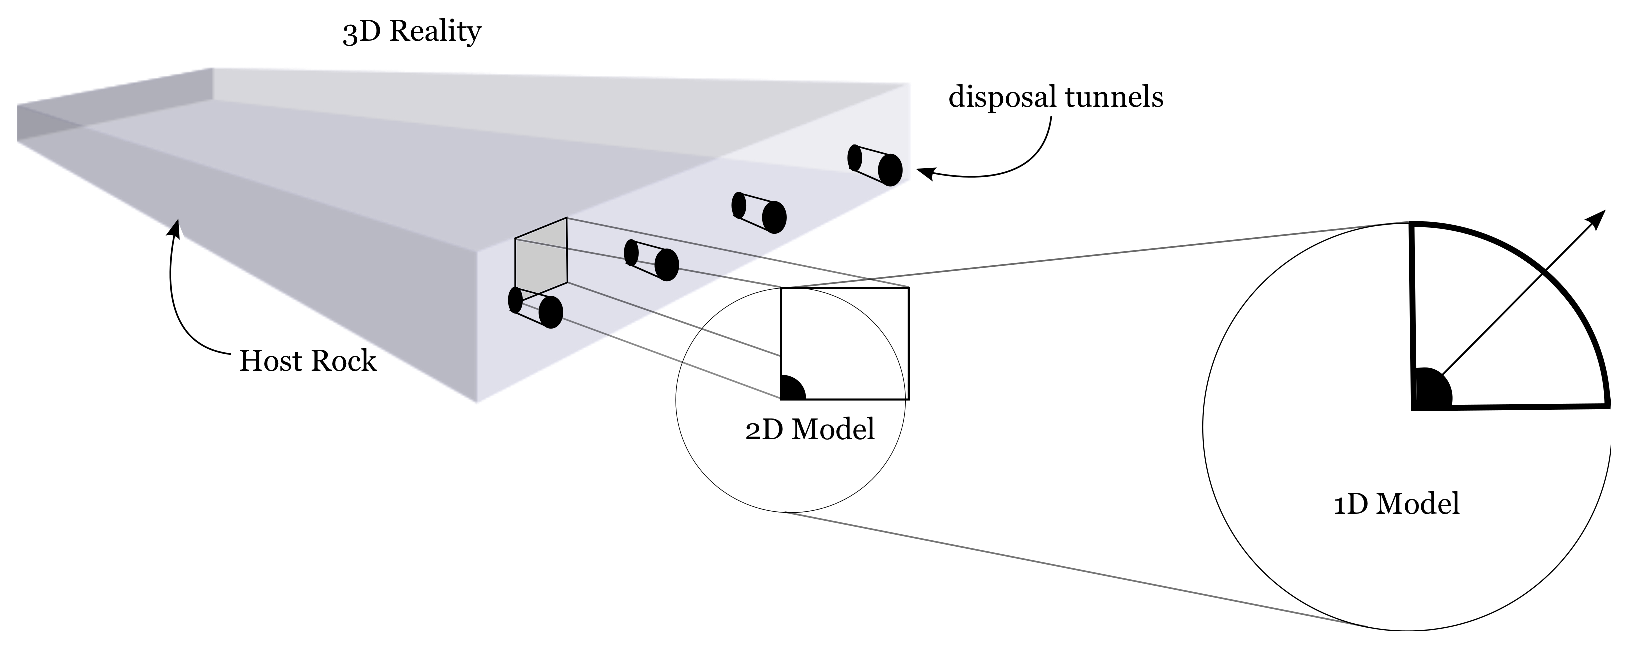
\includegraphics[width=0.9\textwidth]{3dto1d.eps}
    \end{center}
    \caption{Employing the symmetries of the disposal layout can enable lower 
    dimensional models.}
    \label{fig:3dto1d}
  \end{figure}
\end{frame}

\begin{frame}[ctb!]
  \frametitle{Dispersion}
For unidirectional flow, the unidirectional dispersion tensor gives 
\begin{align}
  D_x \frac{\partial^2 C}{\partial x^2} +
  D_y \frac{\partial^2 C}{\partial y^2} +
  D_z \frac{\partial^2 C}{\partial z^2} +
  v_z \frac{\partial C}{\partial z}  = R_f 
  \frac{\partial(nC)}{\partial t}. 
  \label{unidirflow}
\end{align}
\end{frame}

\begin{frame}[ctb!]
  \frametitle{Diffusion}
A special case of uniform flow, no flow, simplifies to the diffusion equation,
\begin{align}
  D_x \frac{\partial^2 C}{\partial x^2} +
  D_y \frac{\partial^2 C}{\partial y^2} +
  D_z \frac{\partial^2 C}{\partial z^2} +
  = R_f 
  \frac{\partial(nC)}{\partial t} .
  \label{diffusion}
\end{align}
\end{frame}

\begin{frame}[ctb!]
  % Precipitation
  \frametitle{Precipitation}
  Elemental solubility limits are based on the maximum concentration of an 
  element which can exist in solution. A limit on concentration in the void 
  volume may be expressed as

    \begin{align} 
      m_{1i}(t)\le v_{1i}(t)C_{sol}
      \intertext{where}
      m_{li} = \mbox{dissolved kg of radionuclide i}\nonumber\\
      v_{li} = \mbox{void volume}\nonumber\\
      C_{sol} = \mbox{solubility limit}\nonumber
    \end{align}
    
\end{frame}




  % Ogata and Banks
\begin{frame}[ctb!]
  \frametitle{One Dimensional Solution with a Constant Concentration Source}
An analytical solution for the one dimensional case with a continuous source 
of constant concentration is known \cite{schwartz_fundamentals_2004}. For the boundary conditions
\begin{align}
  C(0,t) =& C_0
  \intertext{and}
  \frac{\partial C}{\partial z}\Big|_{z=\infty} =& 0
  \label{BCs}
  \intertext{as well as the initial condition }
  C(z,0) =& 0 \mbox{\hspace{2mm}for\hspace{1mm}} z \in (0,\infty),
\end{align}
the Ogata and Banks solution gives
\begin{align}
  C(z,t) =& \frac{C_0}{2}\left[
  \erfc{\left( \frac{z - \frac{v_zt}{R_f} }{2\sqrt{ 
  \frac{D_zt}{R_f} }} \right)} +
  e^{\frac{v_z}{D_z}}
  \erfc{\left( \frac{z+ \frac{v_zt}{R_f} }{2\sqrt{ 
  \frac{D_zt}{R_f} }} \right)}
  \right].
  \label{ogatabanks}
  \intertext{where}
  \erfc(z) =& \frac{2}{\sqrt{\pi}}\int_Z^\infty e^{-t^2}dt. 
\end{align}
\end{frame}



\subsection{Models of Heat Transport}


\begin{frame}[ctb!]
  \frametitle{Heat Limits In Geology}
  % table?
  Important heat limits in materials of the repository restrict loading designs 
  and capacity.
  %        File: heat_tab.tex
%     Created: Thu Aug 04 11:00 AM 2011 C
% Last Change: Thu Aug 04 11:00 AM 2011 C
%
\begin{table}[h!]
  \centering
  \footnotesize{
  \begin{tabular}{|l|r|r|r|r|}
    \multicolumn{5}{c}{\textbf{Thermal Behavior of Various Concepts}}\\
    \hline
    Feature & Clay & Granite & Salt & Deep Borehole \\ 
    \hline
    Buffer Limit $[^{\circ}C]$ & 100 (Fo-Ca) & 100 (Fo-Ca) & 180 & 100 (Fo-Ca) \\ 
    Host Limit $[^{\circ}C]$   & 100 (alteration)  & 200 (cracking) & 180 (brines) & none \\ 
    Conductivity $[\frac{W}{m{\cdot}K}]$ & $1-2$ & $2-4$ & $\sim4$  & $2-4$ \\ 
    Coalesence & yes & no & yes & no \\ 
    \hline
  \end{tabular}
  }
  \label{tab:heat_tab}
\end{table}

\end{frame}

% heat based capacity 
\begin{frame}[ctb!]
  \frametitle{Impact of Repository Designs}
  % lines, points, infinite lines, footprints.
   \input{../report/litrev/footprint_tab.tex}
   \begin{figure}[h!]
     \begin{center}
       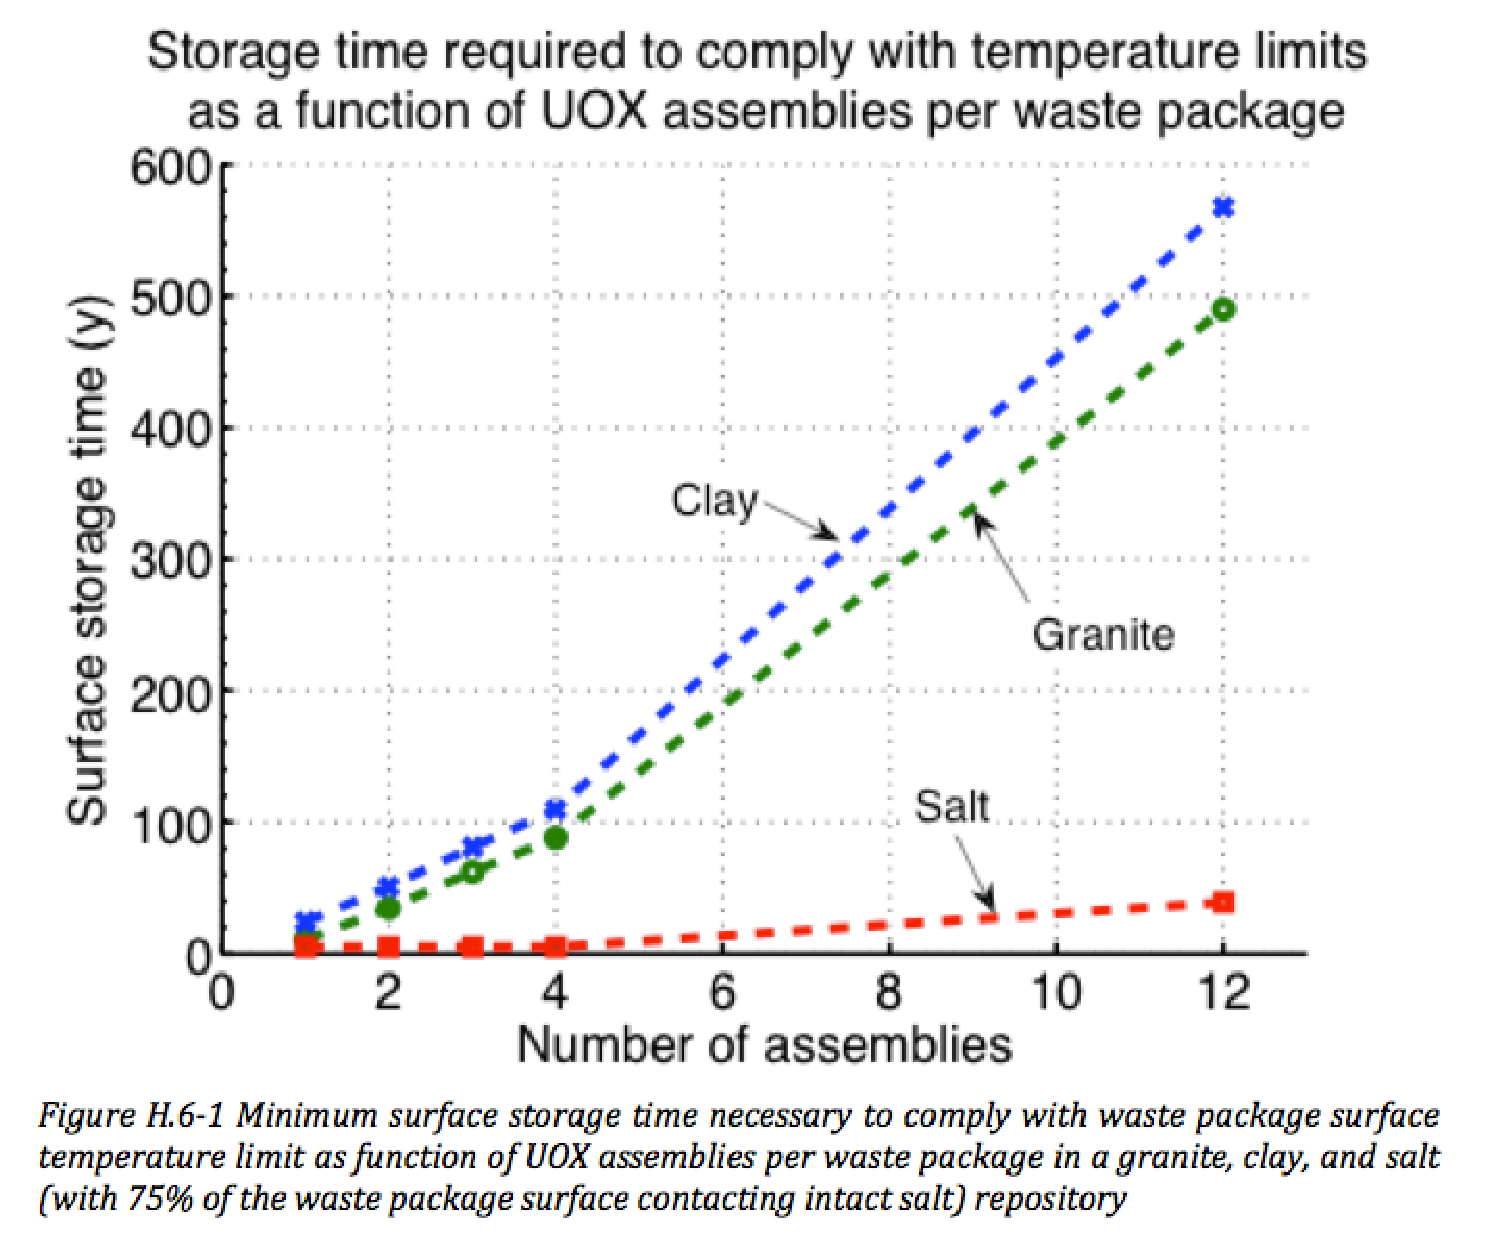
\includegraphics[height=.5\textheight]{./images/llnlGeos.eps}
     \end{center}
     \caption{LLNL has found that the higher heat limit, alcove geometry, and 
     high conductivity in salt allows for earlier loading times.}
     \label{fig:llnlGeos}
   \end{figure}
\end{frame}

% heat based capacity 
\begin{frame}[ctb!]
  \frametitle{Heat Based Capacity}
  % lines, points, infinite lines, footprints.
  \begin{minipage}{0.49\textwidth}
    \begin{figure}[h!]
        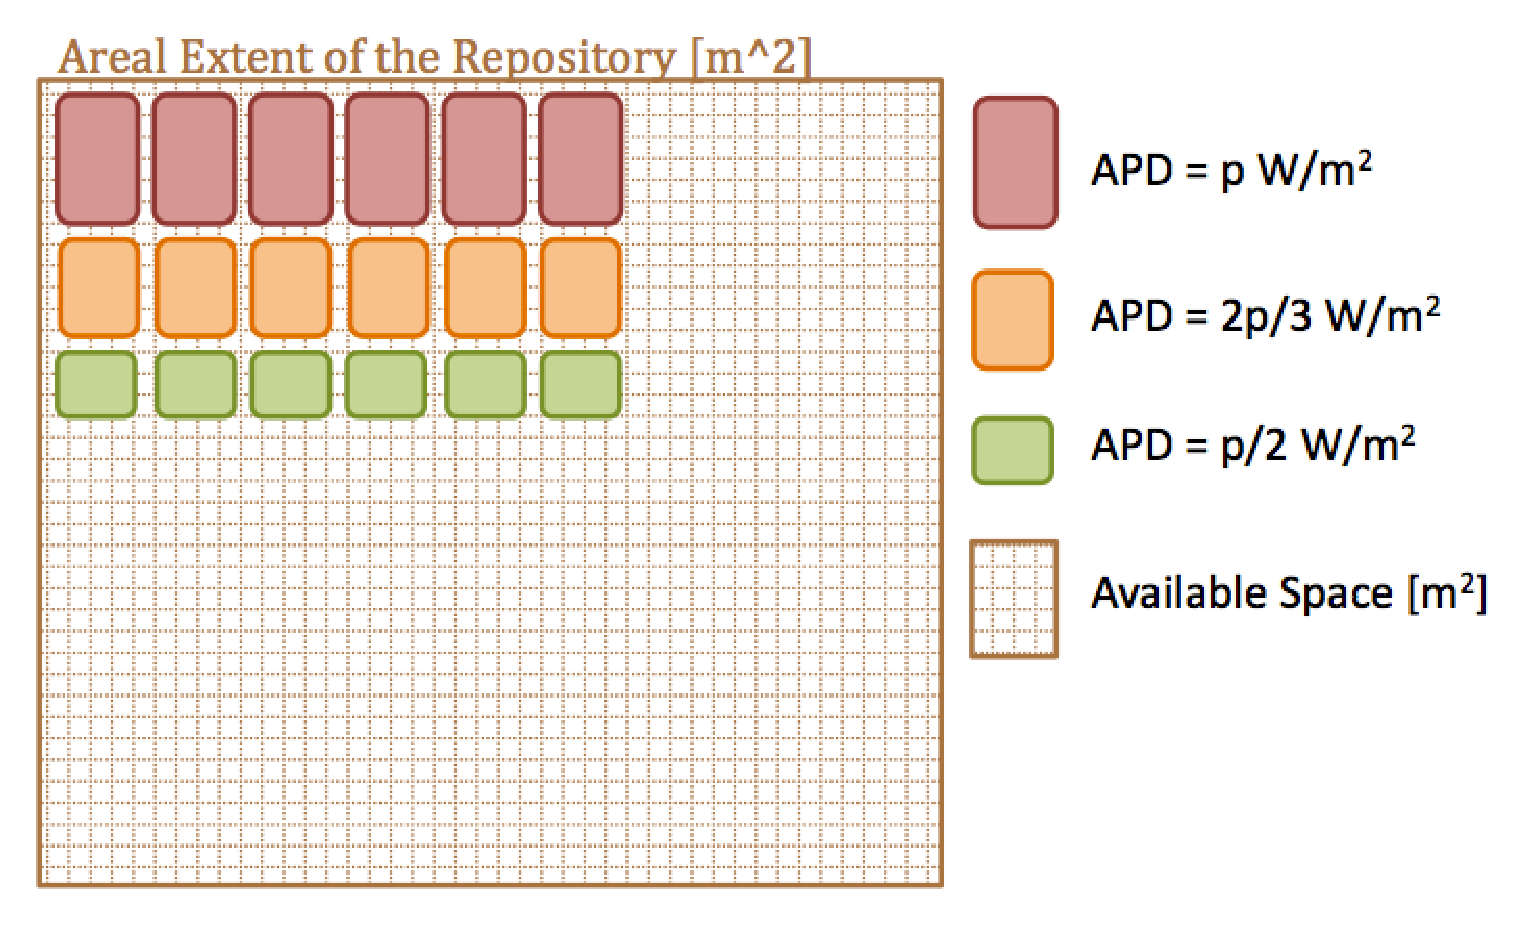
\includegraphics[width=0.9\textwidth]{./images/APD.eps}
      \caption{Areal Power Density (APD) can be used to determine appropriate 
      repository loading for arbitrary waste streams. }
      \label{fig:apd}
  \end{figure}
  \end{minipage}
  \hspace{0.01cm}
  \begin{minipage}{0.49\textwidth}
    Loading is subject to the constraints,
    \footnotesize{
    \begin{align}
      P_{tot} &\le P_{max} \\
      APD_i &\le APD_{max}
      \intertext{where}
      P_{max} &= A\cdot APD_{max}\\ 
      P_{tot} &= \sum_{i=0}^{N}n_i P_i\\ 
      P_i &= \mbox{power of package i}\nonumber\\
      n_i &= \mbox{ith package}\nonumber\\
      N &= \mbox{number of packages}\nonumber\\
      APD_{max} &= \mbox{max areal power density}\nonumber
    \end{align}
    }
  \end{minipage}
\end{frame}

\begin{frame}[ctb!]
  \frametitle{Detailed Techniques}
  % 2d,3d,finite diffs, etc.
  %        File: heat_tab.tex
%     Created: Thu Aug 04 11:00 AM 2011 C
% Last Change: Thu Aug 04 11:00 AM 2011 C
%
\begin{table}[h!]
  \centering
  \footnotesize{
  \begin{tabular}{|l|r|r|r|r|}
    \multicolumn{5}{c}{\textbf{Thermal Behavior of Various Concepts}}\\
    \hline
    Feature & Clay & Granite & Salt & Deep Borehole \\ 
    \hline
    Buffer Limit $[^{\circ}C]$ & 100 (Fo-Ca) & 100 (Fo-Ca) & 180 & 100 (Fo-Ca) \\ 
    Host Limit $[^{\circ}C]$   & 100 (alteration)  & 200 (cracking) & 180 (brines) & none \\ 
    Conductivity $[\frac{W}{m{\cdot}K}]$ & $1-2$ & $2-4$ & $\sim4$  & $2-4$ \\ 
    Coalesence & yes & no & yes & no \\ 
    \hline
  \end{tabular}
  }
  \label{tab:heat_tab}
\end{table}

  Similar heat transport models can be used for all geologies, but are 
  differentiated by material parameters $(c_p, K, \rho)$ and different 
  thermal constraints.
\end{frame}


% SINDA 

\begin{frame}
  \frametitle{ANL model}
  A model created by the UFD team at Argonne national lab using the 
  SINDA{\textbackslash}G heat transport framework employs a lumped parameter 
  model and an optimization loop to arrive at a minimal drift spacing for a 
  given waste stream in agreement with user input thermal limits. 
  \begin{figure}[h!]
    \begin{center}
      \includegraphics[height=.5\textheight]{../report/litrev/sindageom.eps}
    \end{center}
    \caption{Two adjustable geometric dimensions of the ANL model.} 
    \label{fig:sindageom}
  \end{figure}
\end{frame}


\begin{frame}[ctb!]
  \frametitle{Lumped Parameter Technique}
  % resistor diagram
  \begin{figure}[h!]
    \begin{center}
      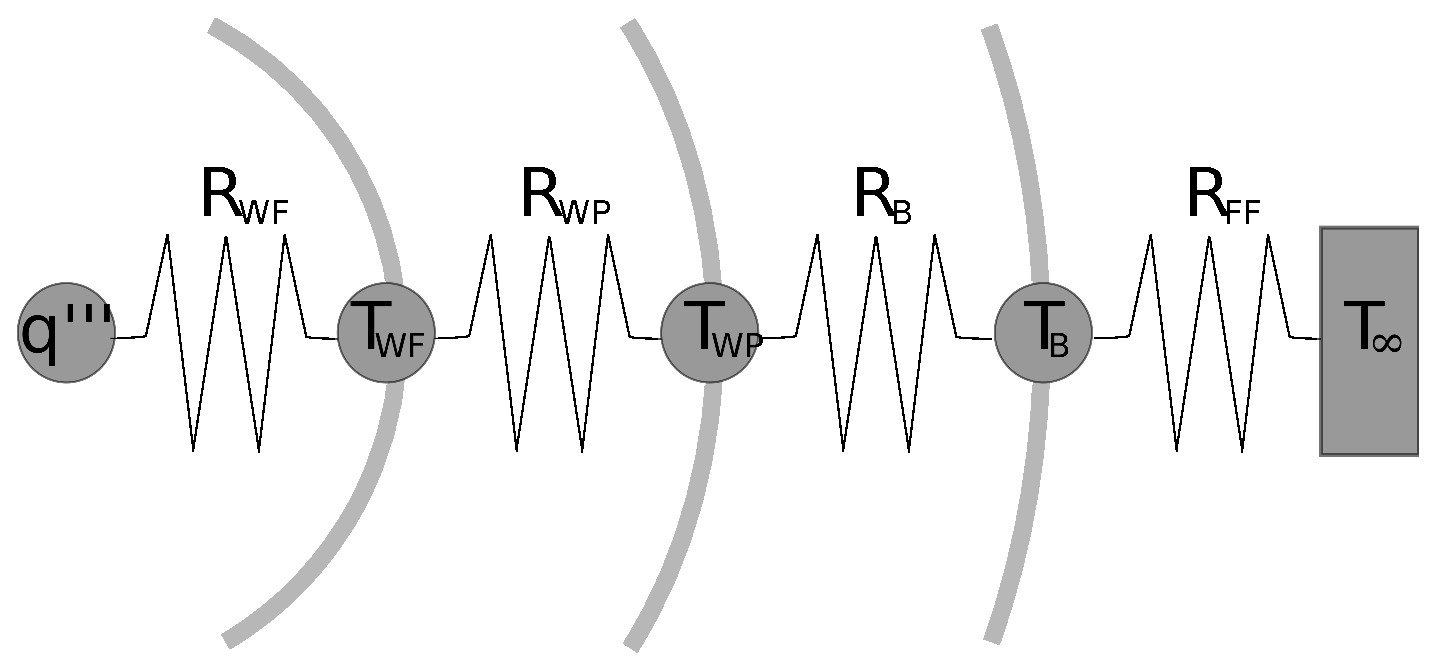
\includegraphics[width=0.9\textwidth]{./images/lumpedParam.eps}
    \end{center}
    \caption{The lumped parameter analogy used for heat transfer can be applied 
    as a one dimensional approximation to the disposal system concept. }
    \label{fig:lumpedParam}
  \end{figure}
\end{frame}


% LLNL

\begin{frame}
  \frametitle{LLNL Model : Geometry}
  \begin{minipage}{0.3\textwidth}
    \begin{figure}[h!]
      \includegraphics[width=\textwidth]{./images/boreholes.eps}
    \end{figure}
    \begin{figure}[h!]
      \includegraphics[width=\textwidth]{./images/vertical.eps}
    \end{figure}
  \end{minipage}
  \hspace{0.01cm}
  \begin{minipage}{0.3\textwidth}
    \begin{figure}[h!]
      \includegraphics[width=\textwidth]{./images/horizontal.eps}
    \end{figure}
    \begin{figure}[h!]
      \includegraphics[width=\textwidth]{./images/alcoves.eps}
    \end{figure}
  \end{minipage}
  \hspace{0.01cm}\large{$=$}\hspace{0.01cm}
  \begin{minipage}{0.3\textwidth}
    \begin{figure}[b]
      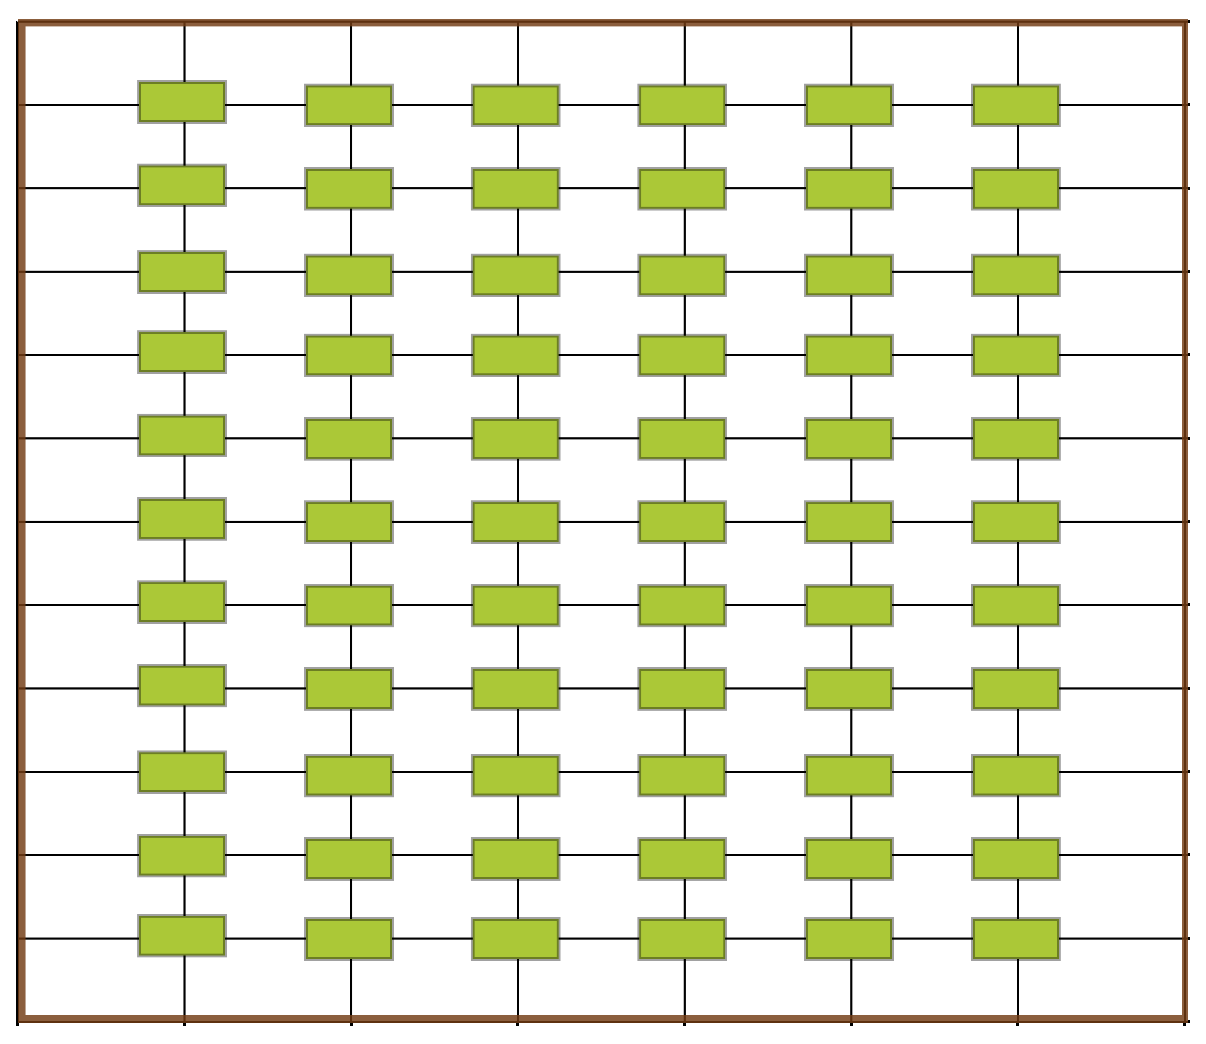
\includegraphics[width=\textwidth]{./images/fullGrid.eps}
    \end{figure}
  \end{minipage}
\end{frame}

\begin{frame}
  \frametitle{LLNL Model : Geometry}
  \begin{figure}[h!]
    \begin{center}
      \includegraphics[width=0.7\textwidth]{./images/llnlConcept.eps}
    \end{center}
    \caption{Vertical, horizontal, alcove, and borehole emplacement layouts can 
    be represented by a line of point sources and adjacent line sources 
    \cite{sutton_investigations_2011}.}
    \label{fig:llnl}
  \end{figure}
\end{frame}

\begin{frame}
  \frametitle{LLNL Model : Solution Strategy}
  \footnotesize{
    LLNL's model is a MathCAD solution of the transient homogeneous 
    conduction equation,
    
    \begin{align}
      \nabla^2T  = \frac{1}{\alpha}\frac{\partial T}{\partial t},
      \label{condGl}
    \end{align}
    
    in which superimposed point and line source solutions approximate the repository 
    layout.
    The solution of this equation at the 
    boundary of the EBS and the waste package is then treated as a boundary condition 
    for the heterogeneous steady state equation, 
    
    \begin{align}
      \dot{q} &= U A_{out} \left( T_{in} - T_{out} \right)
      \label{condGeneral}
      \intertext{where}
      U&=\frac{1}{\sum_{i}R_i}
      \intertext{which, for the detailed EBS becomes}
      U&=\frac{1}{R_{WF}+R_{WP}+R_{buffer}+\cdots}
    \end{align}
    
    which calculates a resulting temperature gradient through the geometry at each 
    point in time for each layer surface, assuming an infinite line source 
    \cite{hardin_generic_2011, sutton_investigations_2011}. 
    }
\end{frame}




\section{Modeling Paradigm}
\subsection{\textsc{Cyclus} Simulator Paradigm}
%||||---------------
\begin{frame}
  \frametitle{Cyclus Modular Architecture and Open Development}
  The combination of modular encapsulation within the software
  architecture and an open development paradigm allows for simulation
  at multiple levels of simulation detail.
\end{frame}
%---------------||||
%||||--------------
\begin{frame}[ctb!]
  \frametitle{Encapsulation}
  \begin{figure}[htbp!]
    \begin{center}
      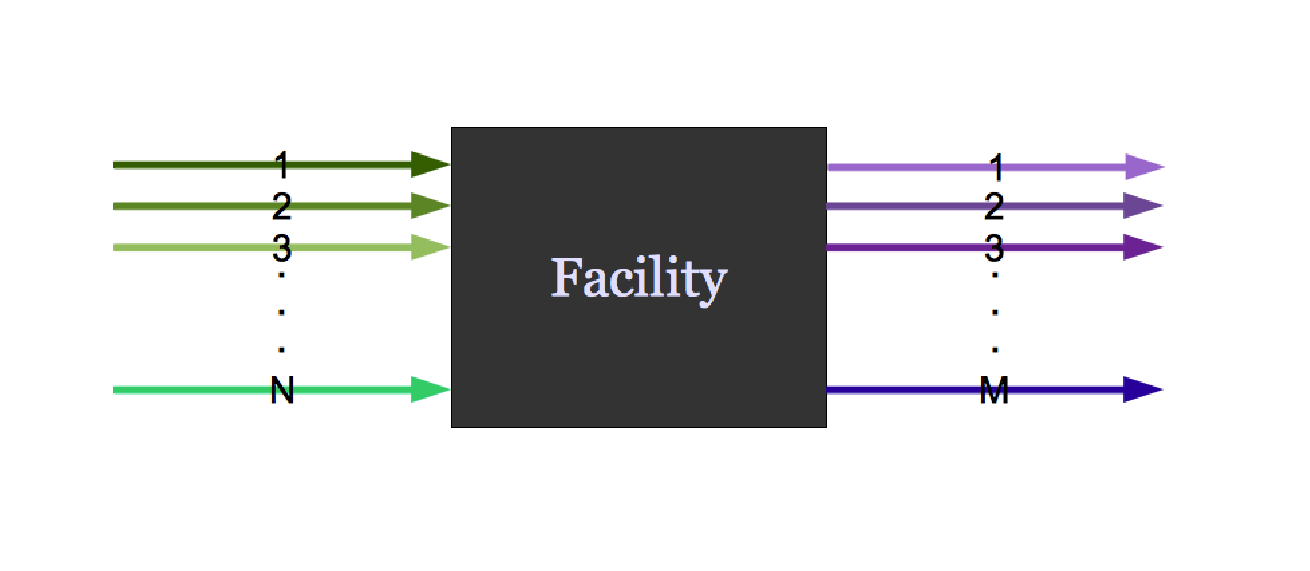
\includegraphics[height=5cm]{facility.eps}
    \end{center}
    \caption{ Regions, Institutions, Facilities, and Markets are all
    black boxes.} 
    \label{fig:sinkfacility}
  \end{figure}
\end{frame}
%---------------||||
%||||---------------
\begin{frame}[ctb!]
  \frametitle{Module Interfaces}
  \begin{figure}[htbp!]
    \begin{center}
      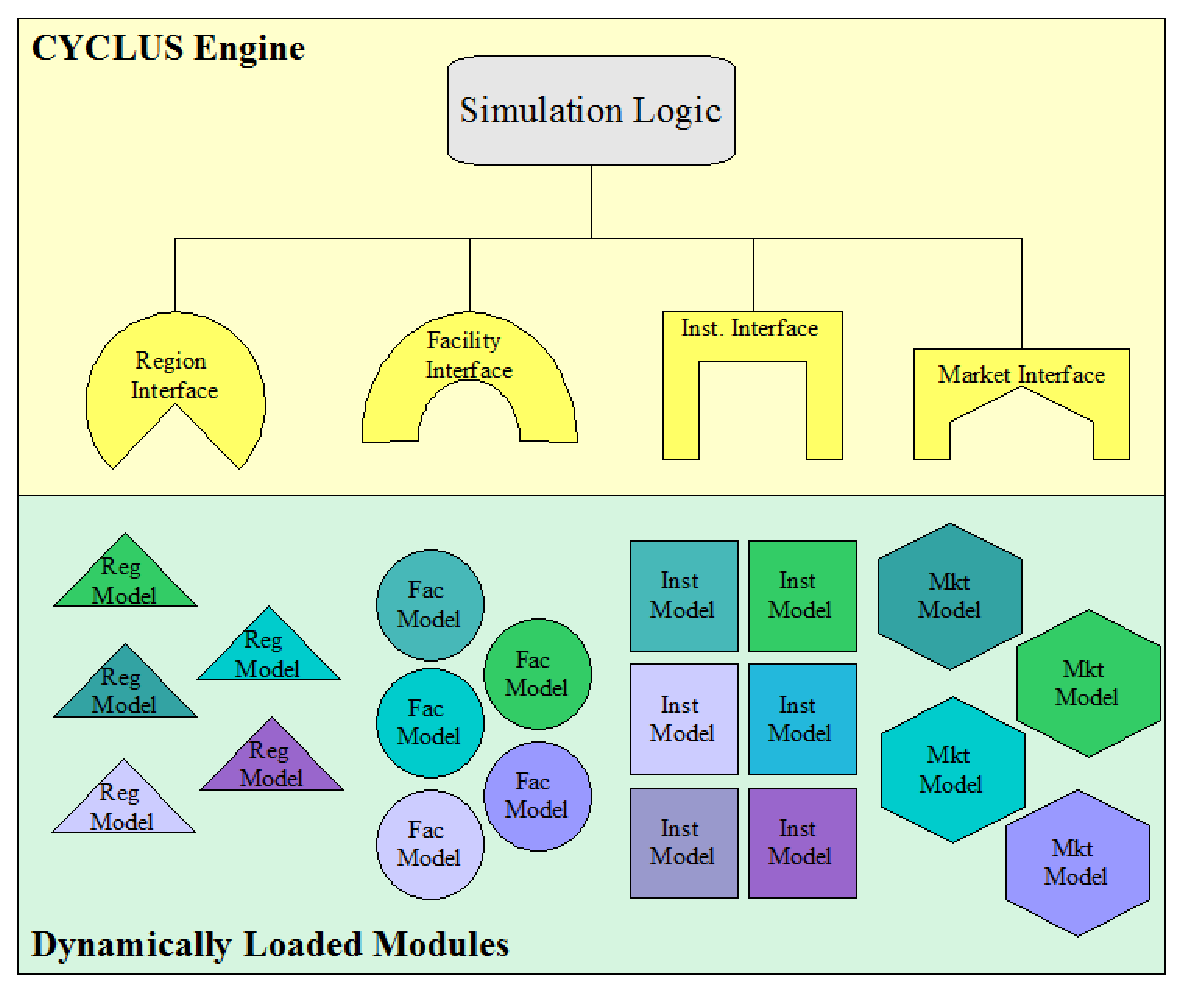
\includegraphics[height=5cm]{interfaces.eps}
    \caption{Well defined model interfaces facilitate model 
    interchange. The user may choose the model at their desired level  
    of detail.}
    \label{fig:interfaces}
    \end{center}
  \end{figure}
\end{frame}
%---------------||||

%||||---------------
\begin{frame}[ctb!]
  \frametitle{Facilities Are Black Boxes}
  \begin{figure}[htbp!]
    \begin{center}
      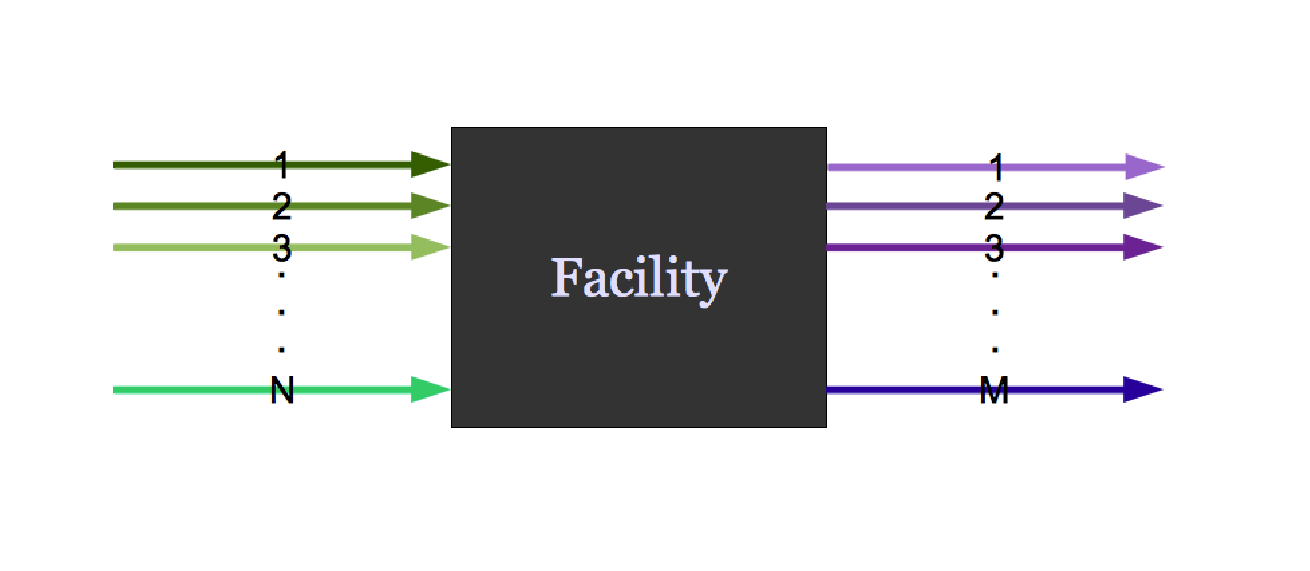
\includegraphics[height=5cm]{facility.eps}
    \end{center}
    \caption{ Each facility in the simulation makes requests and offers 
    to fill its stocks and empty its inventory respectively.  }
    \label{fig:facility}
  \end{figure}
\end{frame}
%---------------||||
%\subsubsection{Example : Market-Facility Interface}
%||||--------------
\begin{frame}[ctb!]
  \frametitle{Facilities Are Black Boxes}
  \begin{figure}[htbp!]
    \begin{center}
      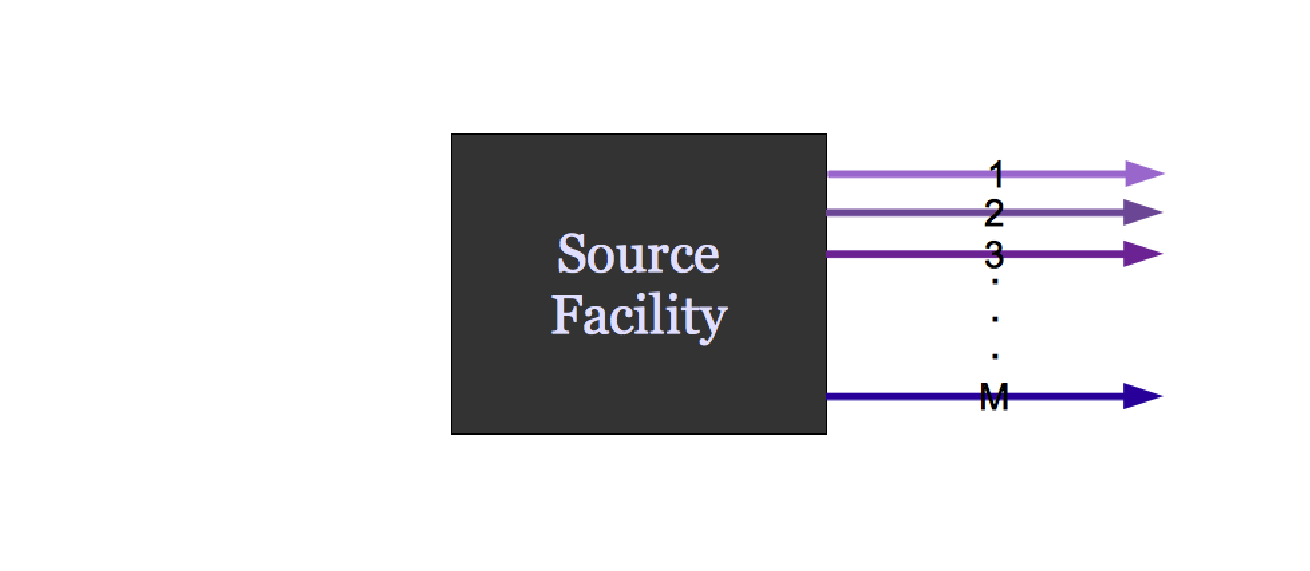
\includegraphics[height=5cm]{sourcefacility.eps}
    \end{center}
    \caption{ A facility might only make offers.} 
    \label{fig:sourcefacility}
  \end{figure}
\end{frame}
%---------------||||
%||||--------------
\begin{frame}[ctb!]
  \frametitle{Facilities Are Black Boxes}
  \begin{figure}[htbp!]
    \begin{center}
      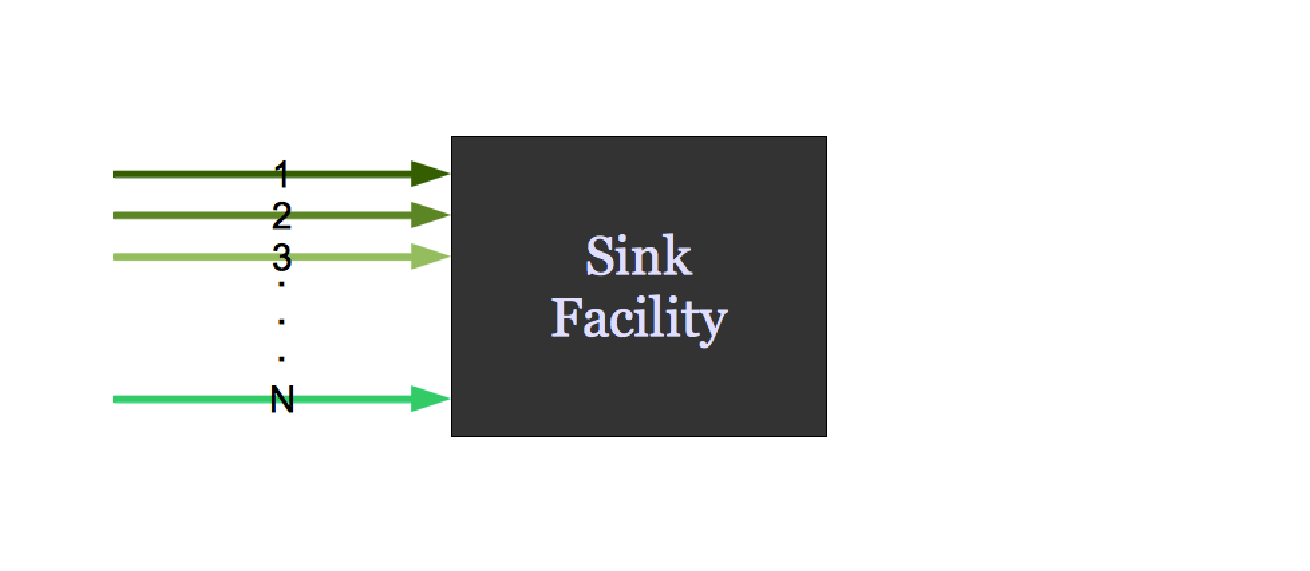
\includegraphics[height=5cm]{sinkfacility.eps}
    \end{center}
    \caption{ A facility might only make requests.} 
    \label{fig:sinkfacility}
  \end{figure}
\end{frame}
%---------------||||
%||||--------------
\begin{frame}[ctb!]
  \frametitle{Each Commodity is Associated with a Market}
  \begin{figure}[htbp!]
    \begin{center}
      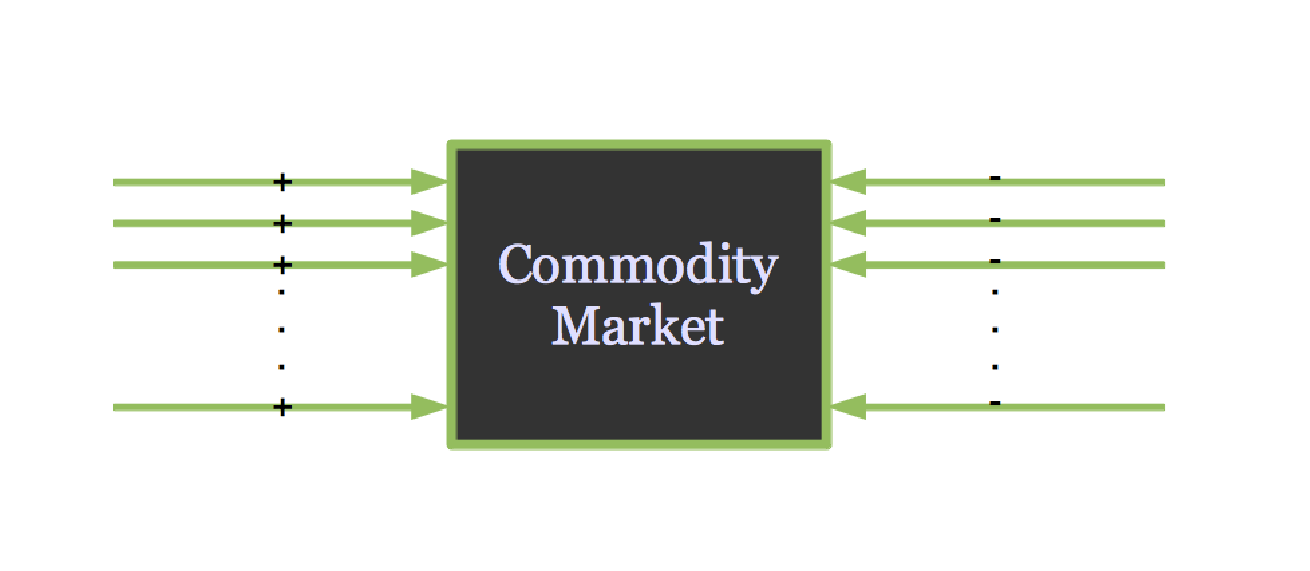
\includegraphics[height=5cm]{market.eps}
    \end{center}
    \caption{ A market receives offers and requests concerning its 
    commodity. } 
    \label{fig:market}
  \end{figure}
\end{frame}
%---------------||||
%||||--------------
\begin{frame}[ctb!]
  \frametitle{The Market Solves the Matching Problem}
  \begin{figure}[htbp!]
    \begin{center}
      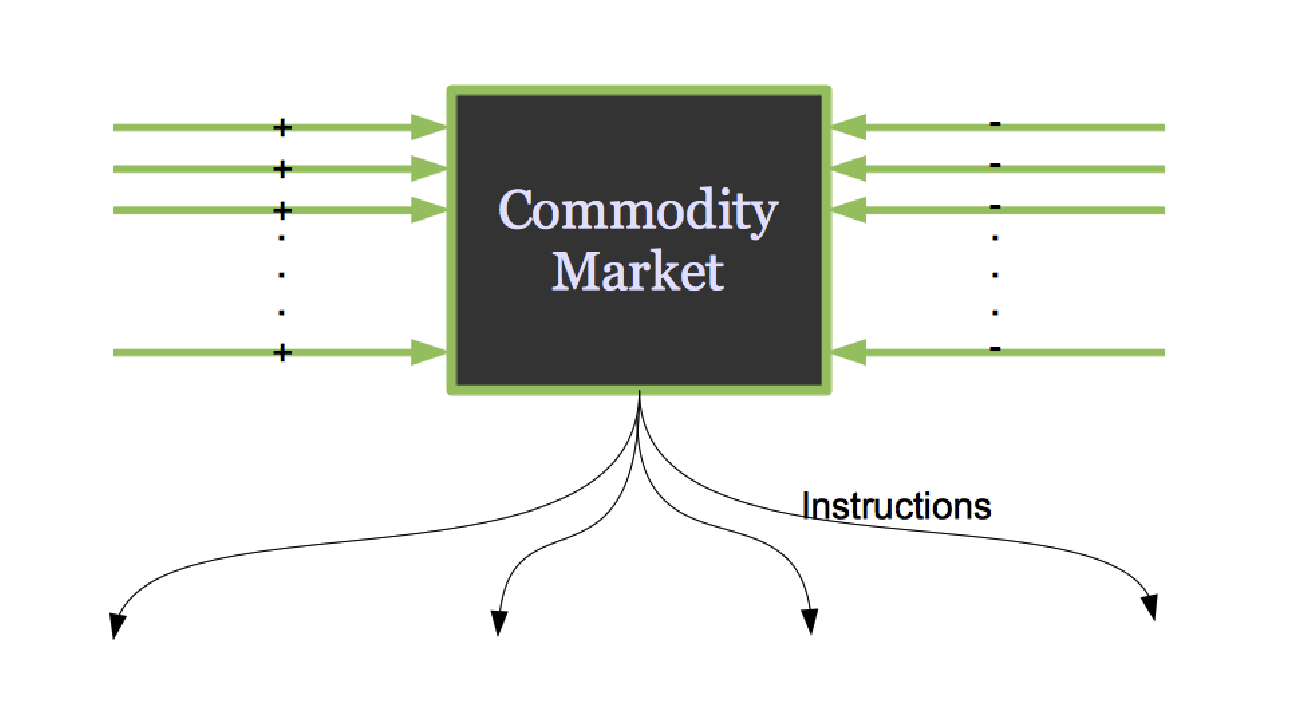
\includegraphics[height=5cm,width=8cm]{instructions.eps}
    \end{center}
    \caption{ When the Market's arbitrary algorithm solves the 
    matching problem, the Market sends instructions to the offering 
    facilities.} 
    \label{fig:instructions}
  \end{figure}
\end{frame}
%---------------||||
%||||--------------
\begin{frame}[ctb!]
  \frametitle{A Simple Example}
  \begin{figure}[htbp!]
    \begin{center}
      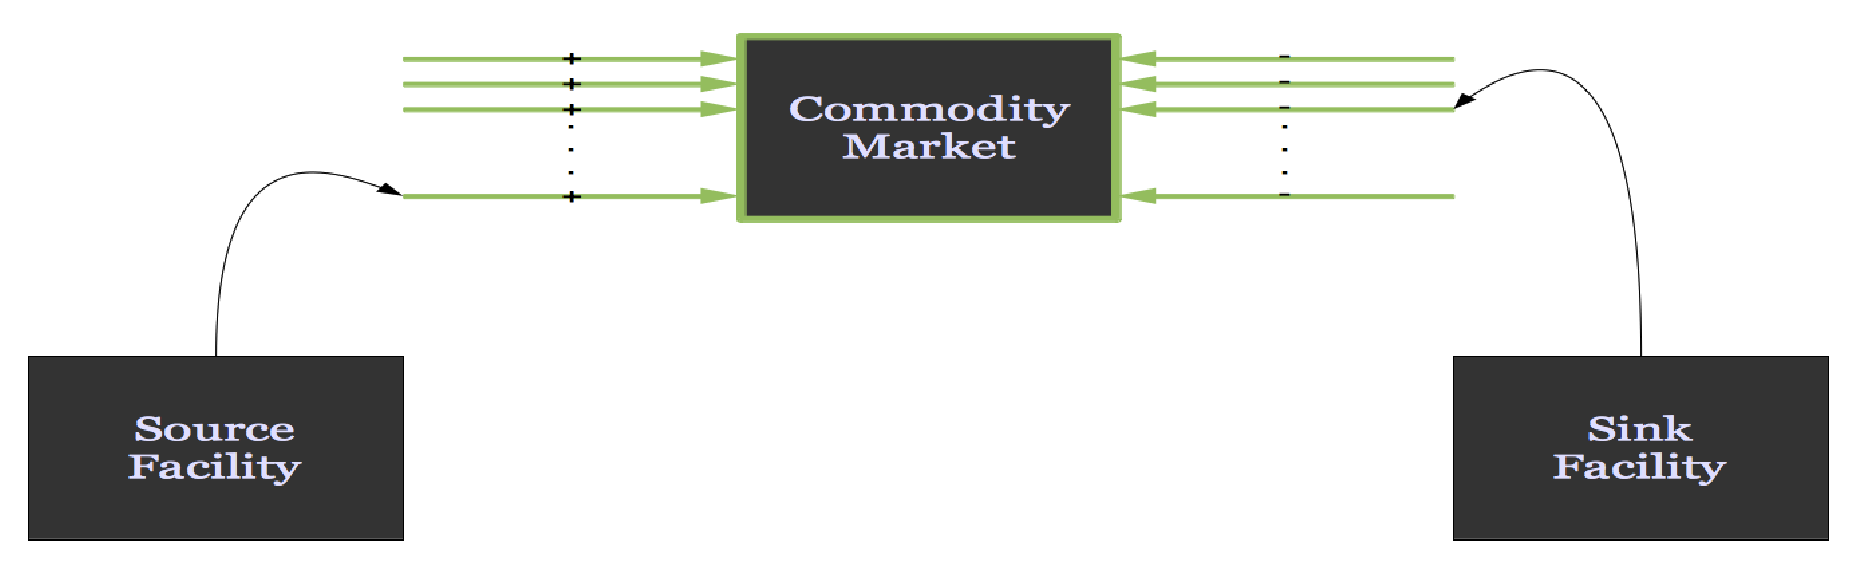
\includegraphics[height=5cm, width=8cm]{offreq.eps}
    \end{center}
    \caption{ The source sends an offer and the sink sends a request.} 
    \label{fig:offreq}
  \end{figure}
\end{frame}
%---------------||||
%||||--------------
\begin{frame}[ctb!]
  \frametitle{A Simple Example}
  \begin{figure}[htbp!]
    \begin{center}
      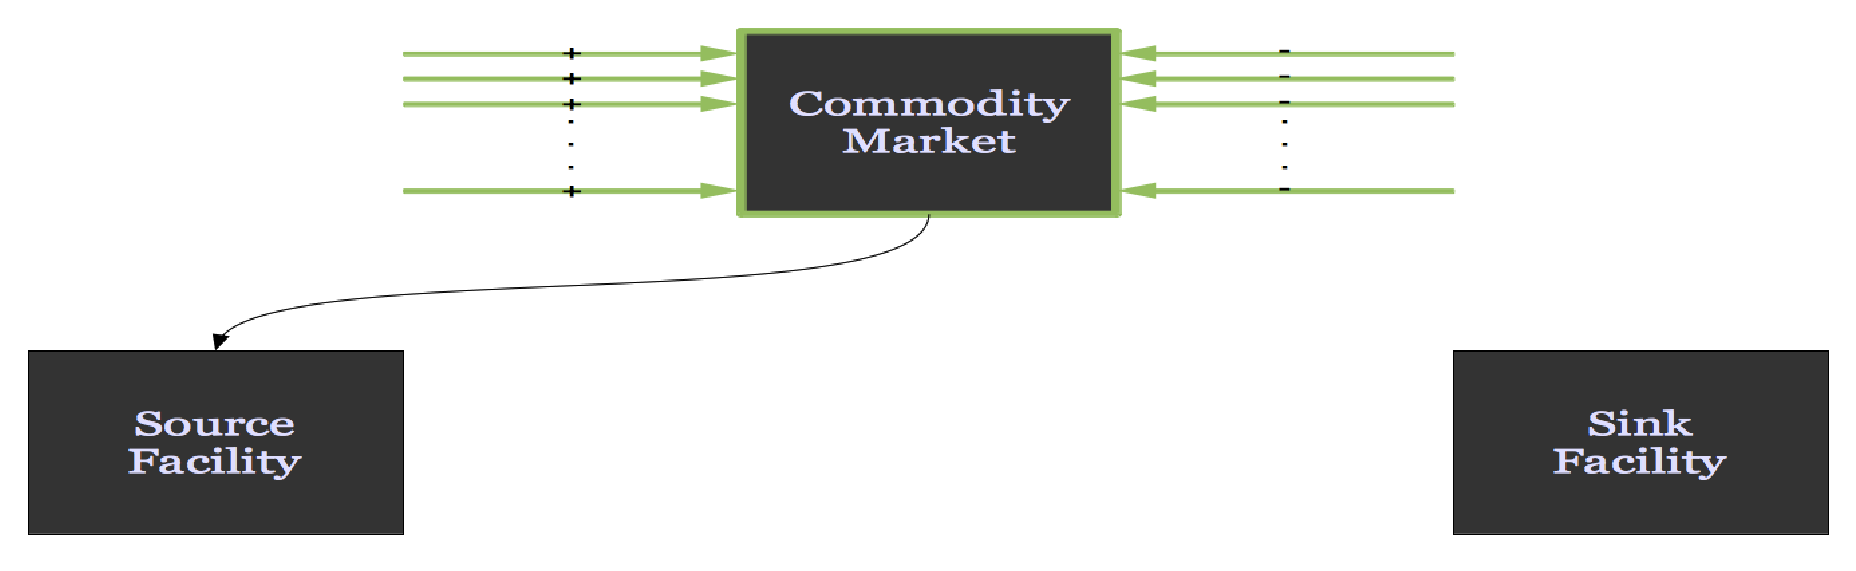
\includegraphics[height=5cm, width=8cm]{transmess.eps}
    \end{center}
    \caption{ The Market solves the problem and instructs the source 
    facility to send a certain amount to the sink facility.} 
    \label{fig:transmess}
  \end{figure}
\end{frame}
%---------------||||
%||||--------------
\begin{frame}[ctb!]
  \frametitle{A Simple Example}
  \begin{figure}[htbp!]
    \begin{center}
      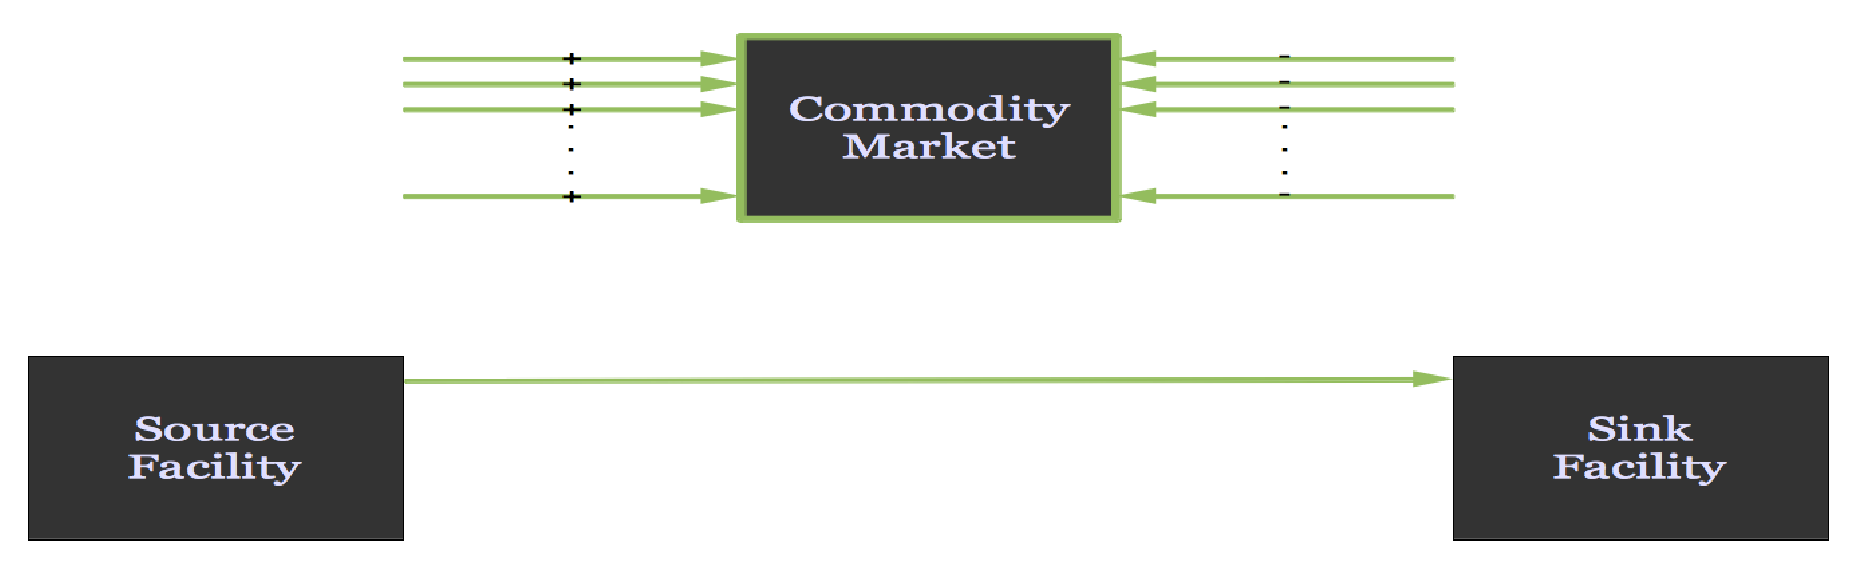
\includegraphics[height=5cm, width=8cm]{trans.eps}
    \end{center}
    \caption{ The source facility sends the material directly to the 
    sink facility.} 
    \label{fig:trans}
  \end{figure}
\end{frame}
%---------------||||
%||||---------------
\begin{frame}[ctb!]
  \frametitle{This Market Model Scales for Complex Systems}
  \begin{figure}[htbp!]
    \begin{center}
      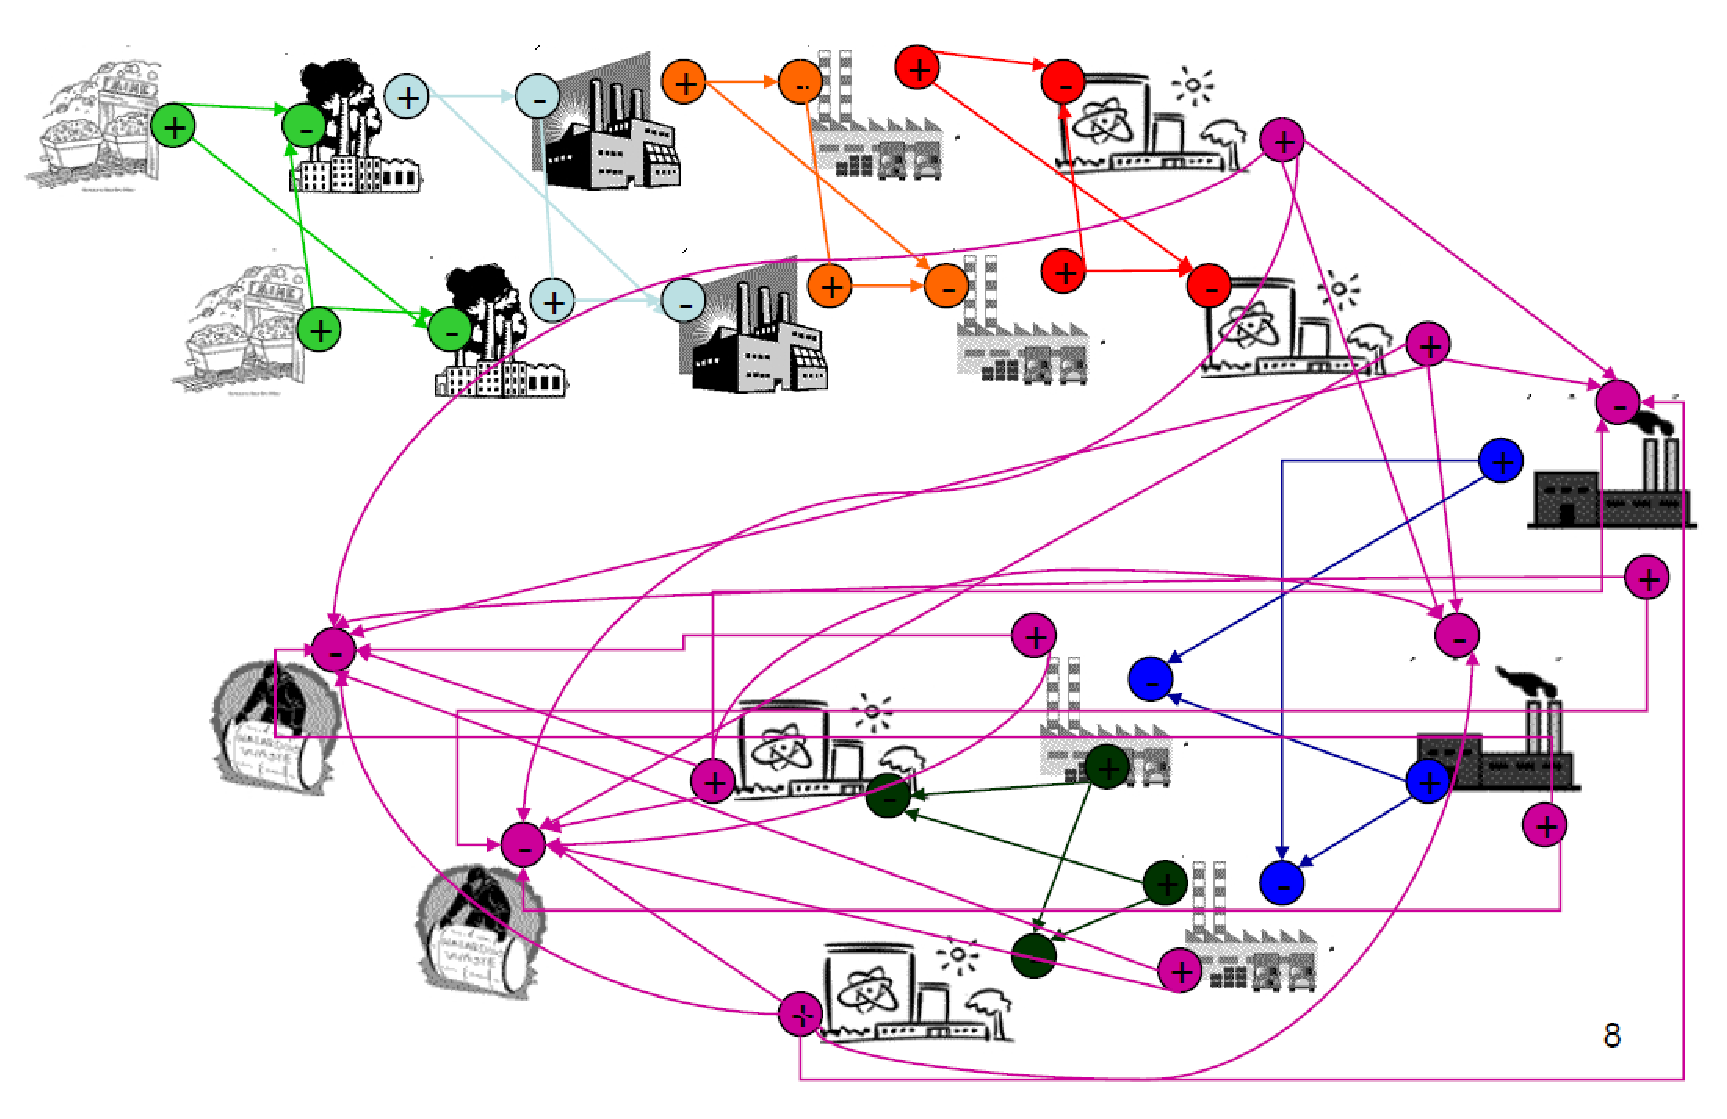
\includegraphics[height=6cm]{materials.eps}
    \end{center}
    \caption{Well designed interfaces and strict encapsulation support 
    scalability of the Market-based simulation paradigm 
    \cite{oliver_geniusv2:_2009}}
    \label{fig:materials}
  \end{figure}
\end{frame}
%---------------||||

%\subsubsection{Extensibility}
%||||---------------
\begin{frame}
  \frametitle{Dynamic Module Loading : Developer}
  With a dynamic, plug-in implementation, the simulation logic is 
  independent of the available models and models are loaded as shared 
  libraries at runtime. 

  \begin{figure}[htbp!]
    \begin{center}
      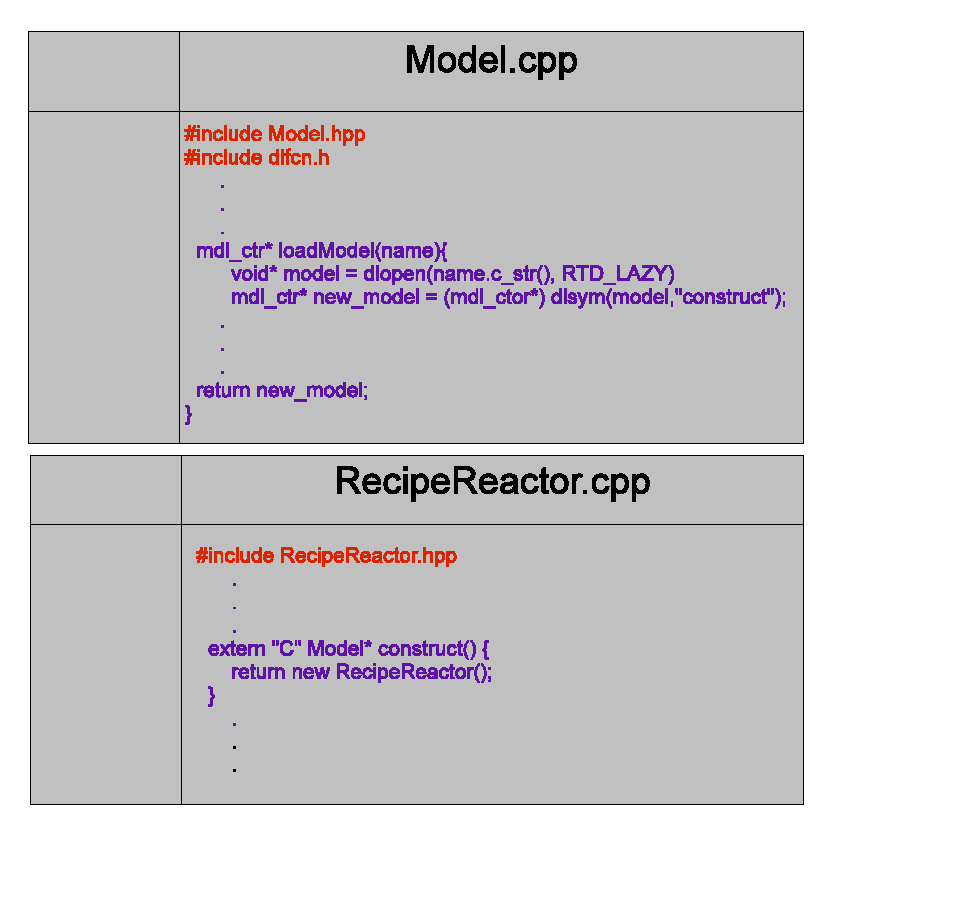
\includegraphics[height=5.5cm]{developer.eps}
    \end{center}
    \caption{Dynamic c library loading separates simulation logic from 
    knowledge of available models, supporting extensions by developers 
    with minimal lines of code.}
    \label{fig:xmlinput}
  \end{figure}

\end{frame}
%---------------||||
%||||---------------
\begin{frame}[ctb!]
  \frametitle{Dynamic Module Loading : User}
  With a dynamic, plug-in implementation, the simulation logic is 
  independent of the available models and models are loaded as shared 
  libraries at runtime. 

  \begin{figure}[htbp!]
    \begin{center}
      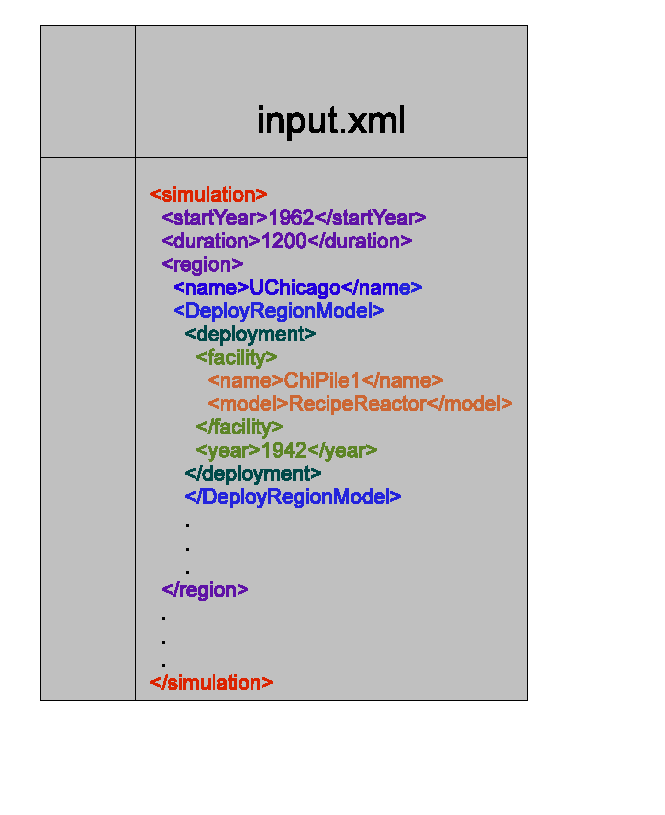
\includegraphics[height=5.5cm]{user.eps}
    \end{center}
    \caption { XML input parsing and a relaxNG schema provide 
    a simplified XML interface is available for the end
    user to define available module implementations.  }
    \label{fig:xmlinput}
  \end{figure}

\end{frame}
%---------------||||

%||||---------------
\begin{frame}[ctb!]
  \frametitle{Open Source Repository}
    This open source repository provides a centralized location for 
    documentation, developer history, and unhindered developer access.
  \begin{figure}[htbp!]
    \begin{center}
      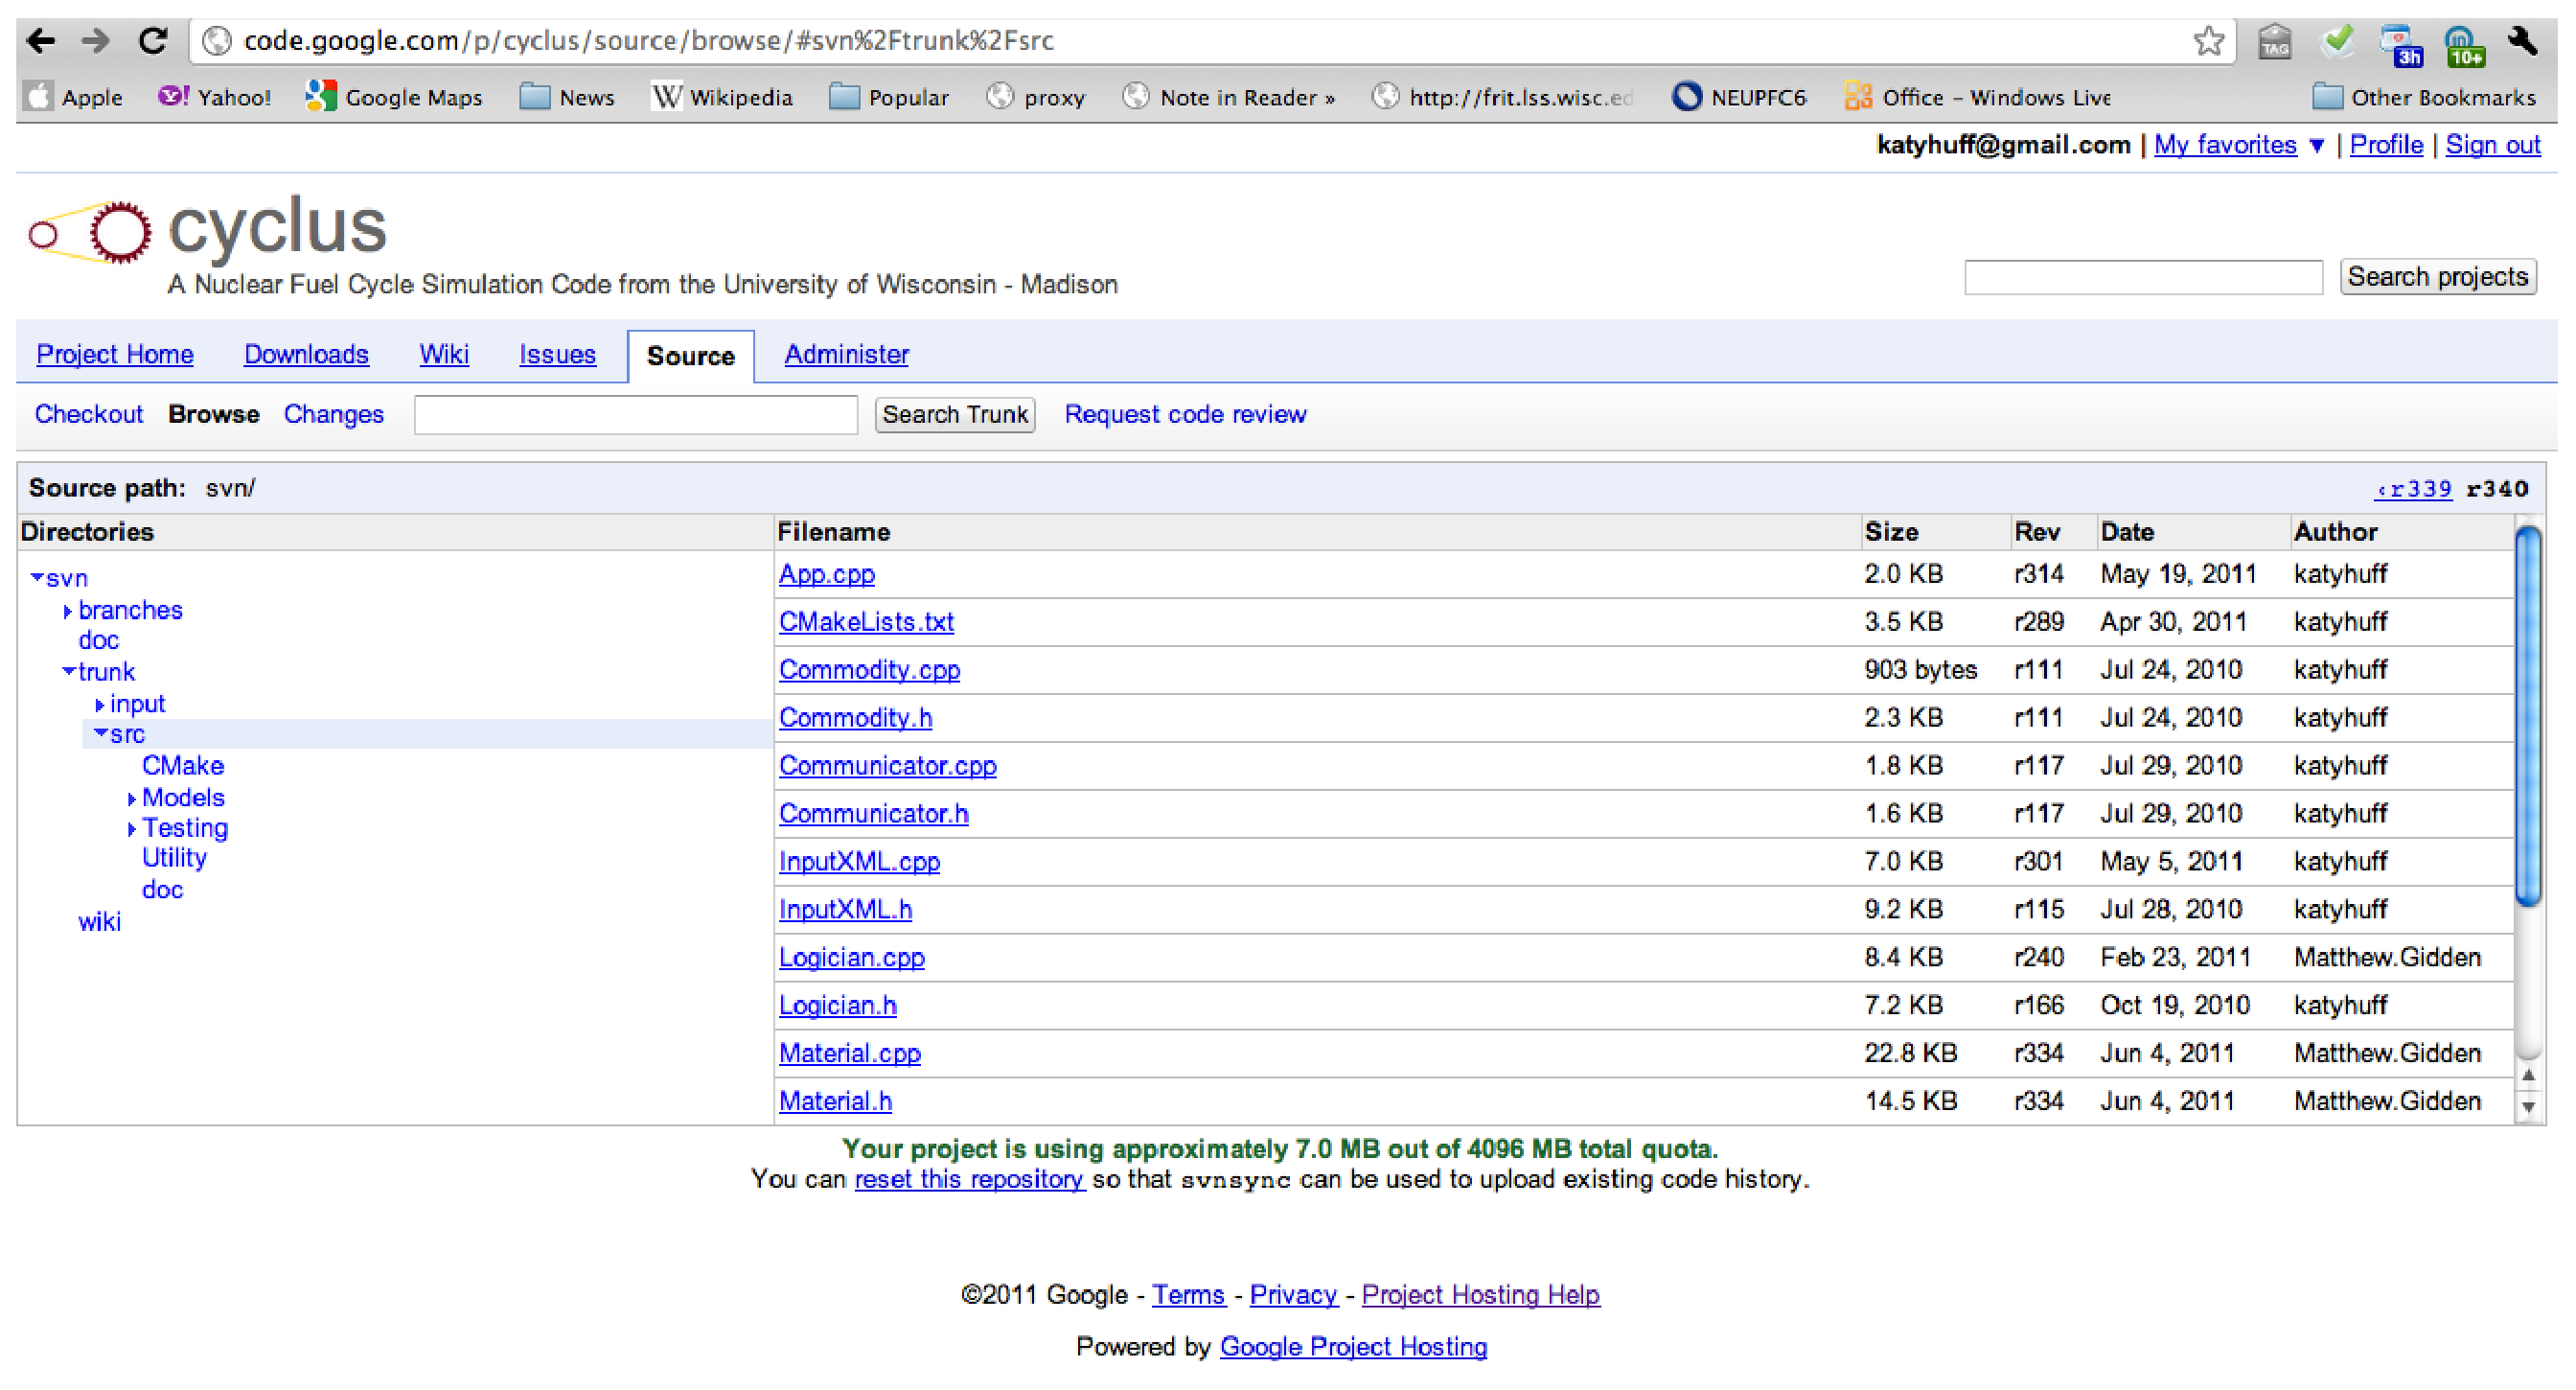
\includegraphics[height=6cm]{source.eps}
    \end{center}
    \caption{The current source code, complete revision history, and 
    documentation are made available for download and contribution 
    online. }
    \label{fig:open}
  \end{figure}
\end{frame}
%---------------||||
%||||---------------
\begin{frame}[ctb!]
  \frametitle{ `Modified Open' Source}
  \begin{figure}[hbtp!]
    \begin{center}
      
\includegraphics[height=6cm]{security.eps}
    \end{center}
    \caption{License, architecture, and development paradigm allow 
    varying levels of code sharing and data security.}
    \label{fig:security}
  \end{figure}
\end{frame}
%---------------||||
%\subsubsection{Quality Control}
%||||---------------
\begin{frame}[ctb!]
  \frametitle{Version Control}
    This open source repository employs a version control system 
     for provenance, developer access, and reproducibility of results.
  \begin{figure}[htbp!]
    \begin{center}
      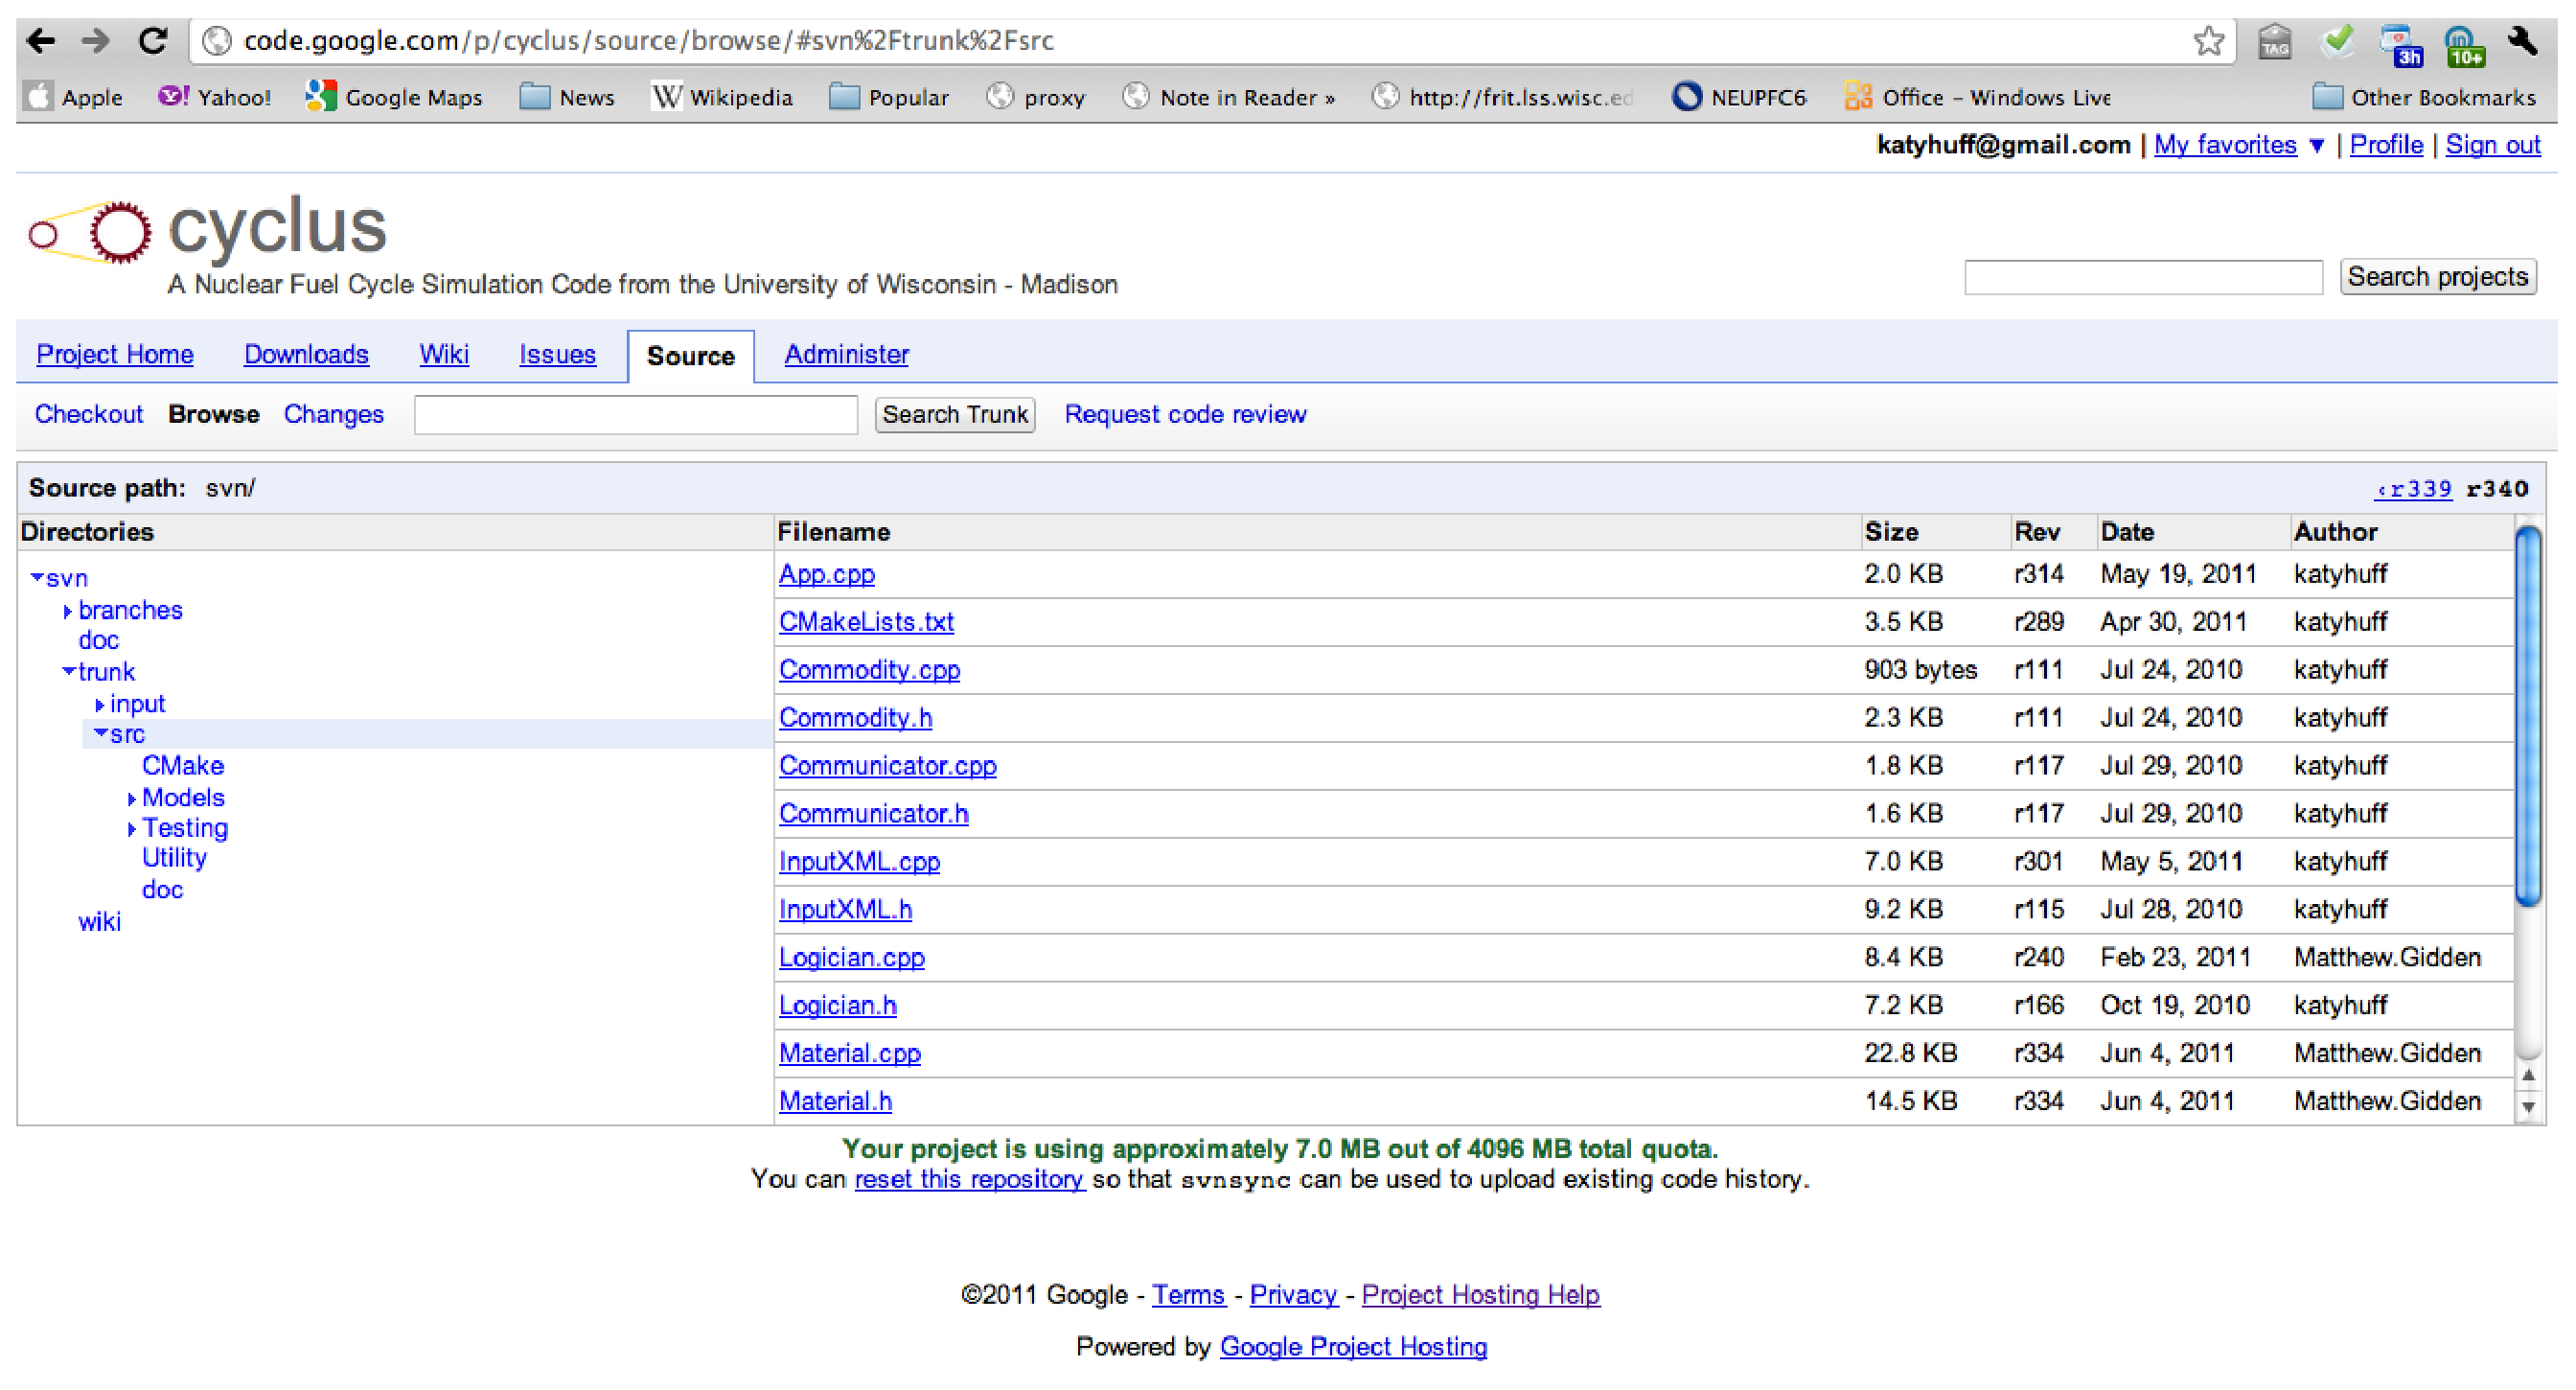
\includegraphics[height=6cm]{source.eps}
    \end{center}
    \caption{The current source code, commit messages, and complete 
    revision history is recorded and available in the repository.}
    \label{fig:source}
  \end{figure}
\end{frame}
%---------------||||

\subsection{Repository Modeling Paradigm}


\begin{frame}[ctb!]
  \frametitle{Nested Components}
  \begin{figure}[h!]
    \begin{center}
      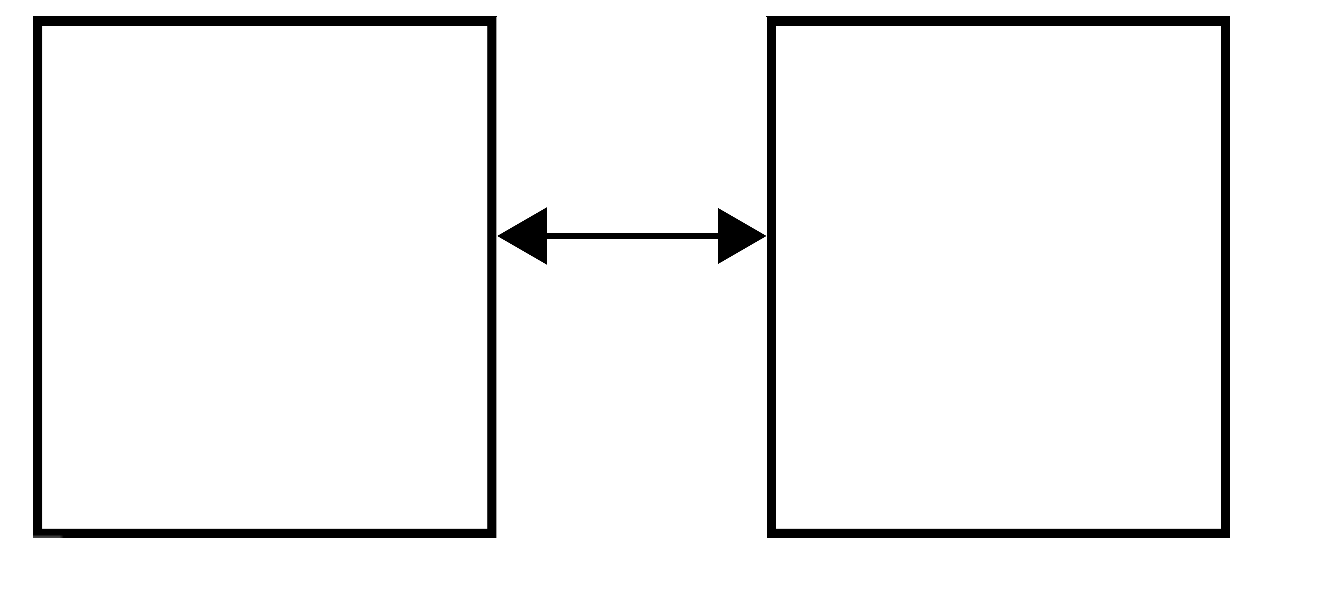
\includegraphics[width=\textwidth]{../report/chapters/paradigm/flow.eps}
    \end{center}
    \caption{The nested components supply thermal flux and concentration 
    information to each other at the boundaries.}
    \label{fig:flow}
  \end{figure}
\end{frame}



\begin{frame}[ctb!]
  \frametitle{Mixed Cell : Permeable Porous Medium}
  % Waste Form
  \begin{figure}[h!]
    \begin{center}
      \includegraphics[height=.6\textwidth]{../report/chapters/future/contaminated1.eps}
    \end{center}
  \end{figure}
\end{frame}

\begin{frame}[ctb!]
  \frametitle{Mixed Cell : Permeable Porous Medium with Degradation}
  % Waste Form
  \begin{figure}[h!]
    \begin{center}
      \includegraphics[height=.6\textwidth]{../report/chapters/future/contaminated.eps}
    \end{center}
  \end{figure}
\end{frame}

\begin{frame}
  \frametitle{Nested Components}
  \begin{itemize}
    \item Waste Form
      \begin{itemize}
        \item Mixed Cell 
        \item with Rate Based Degradation Model
        \item and solubility limits
        \item Data for various waste forms
      \end{itemize}
    \item Waste Package
      \begin{itemize}
        \item Rate Based Failure Model
        \item Data for various waste packages
      \end{itemize}
    \item Buffer
      \begin{itemize}
        \item Mixed Cell 
        \item with Rate Based Degradation Model
        \item Data for various buffers
      \end{itemize}
    \item Geology
      \begin{itemize}
        \item Solute transport model
        \item Data for various geologic media
      \end{itemize}
  \end{itemize}
\end{frame}


\section{Proposed Work}
\subsection{Demonstration Case}


\begin{frame}[ctb!]
  \frametitle{Demonstration Case : Code Development}
  Empty Concept

  Interfaces, information passing, module loading. Not in that order.

  Information passing tests, Database writing tests, module loading tests.
\end{frame}

\subsection{Base Case}


\begin{frame}
  \frametitle{Base Case : Nested Components}
  \begin{itemize}
    \item Waste Form
      \begin{itemize}
        \item Mixed Cell with  Rate Based Degradation Model
        \item Glass and UOx Data
      \end{itemize}
    \item Waste Package
      \begin{itemize}
        \item Rate Based Failure Model
        \item Steel and Copper Data
      \end{itemize}
    \item Buffer
      \begin{itemize}
        \item Mixed Cell with  Rate Based Degradation Model
        \item Bentonite (Fo-Ca), Salt, and Cement Data
      \end{itemize}
    \item Geology
      \begin{itemize}
        \item Ogata and Banks 1D Permeable Porous Medium Solute Transport
        \item Data for Clay, Granite, Salt, and Crystalline Basement
      \end{itemize}
  \end{itemize}
\end{frame}

\begin{frame}[ctb!]
  \frametitle{Base Case : Components}
  \begin{figure}[h!]
      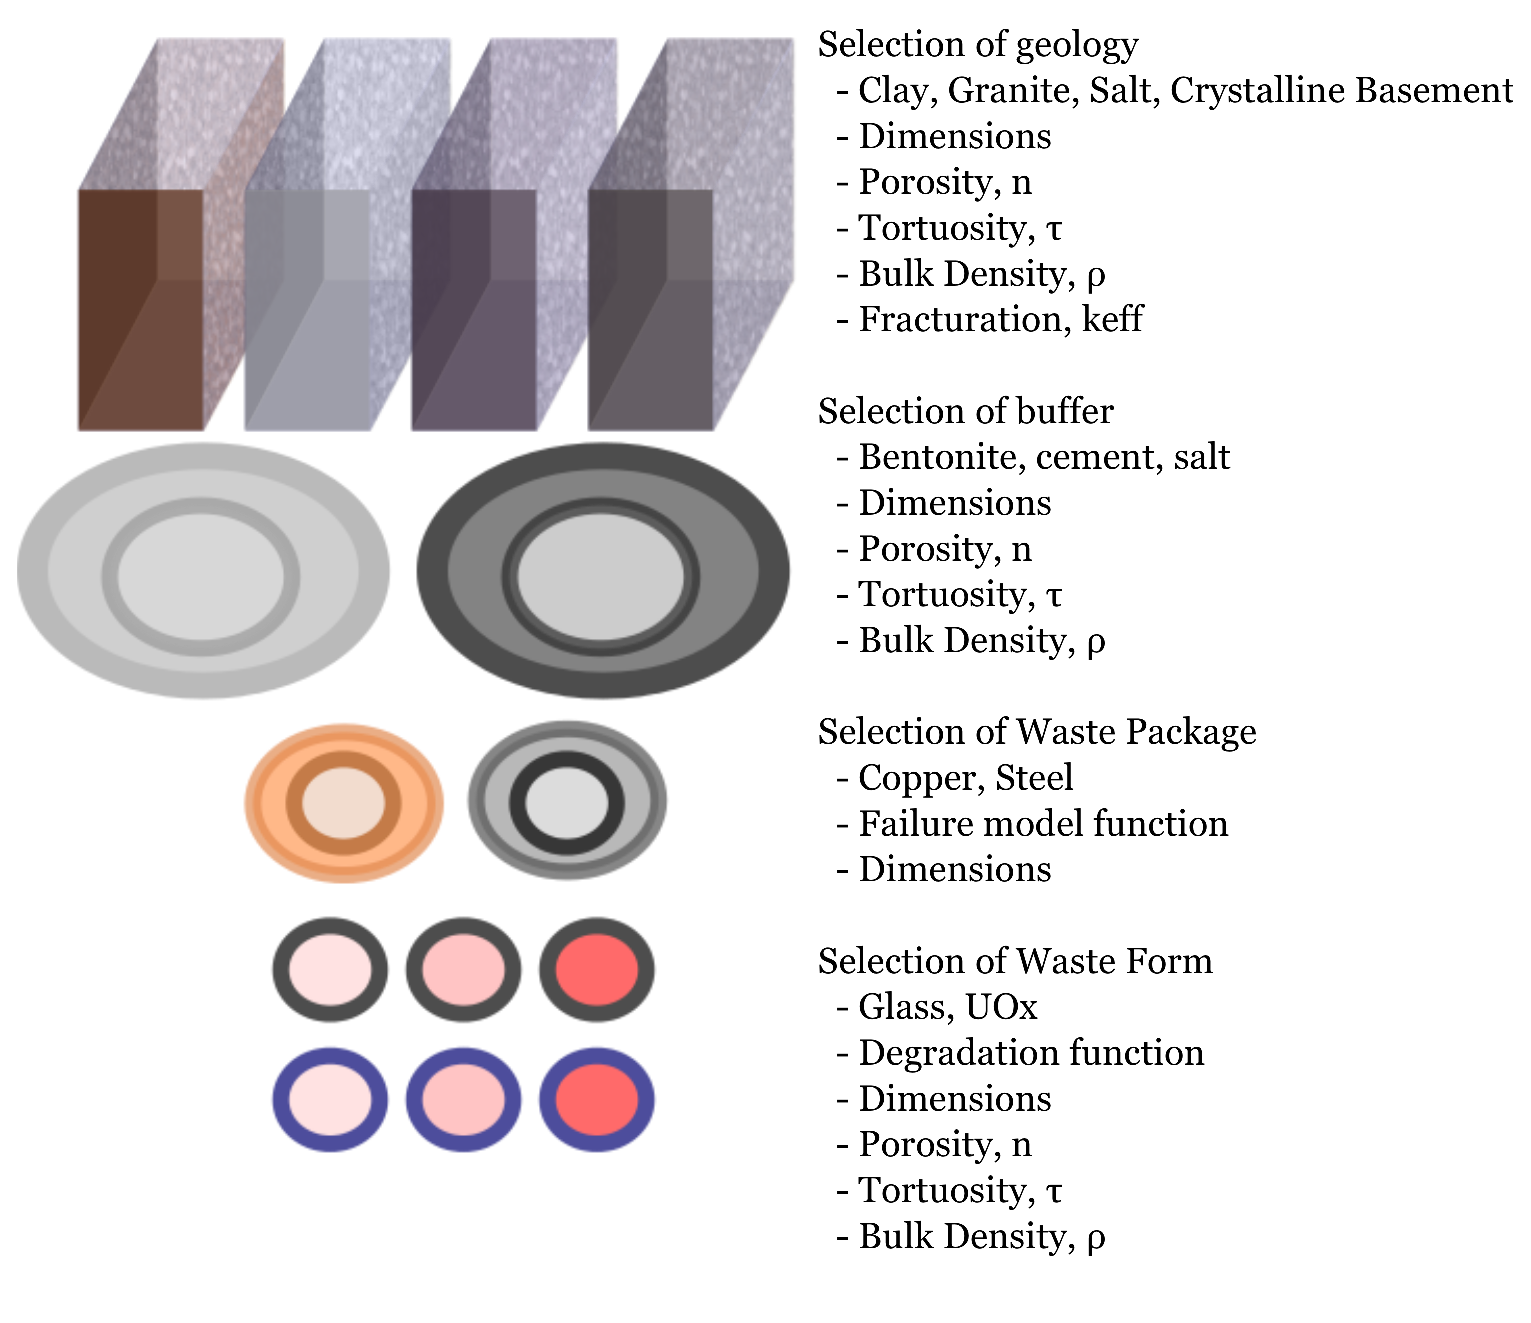
\includegraphics[height=0.8\textheight]{./images/components.eps}
  \end{figure}
\end{frame}

\begin{frame}[ctb!]
  \frametitle{Base Case : Waste Form Abstraction}
  \begin{minipage}{0.45\textwidth}
    \begin{figure}[h!]
      \begin{center}
        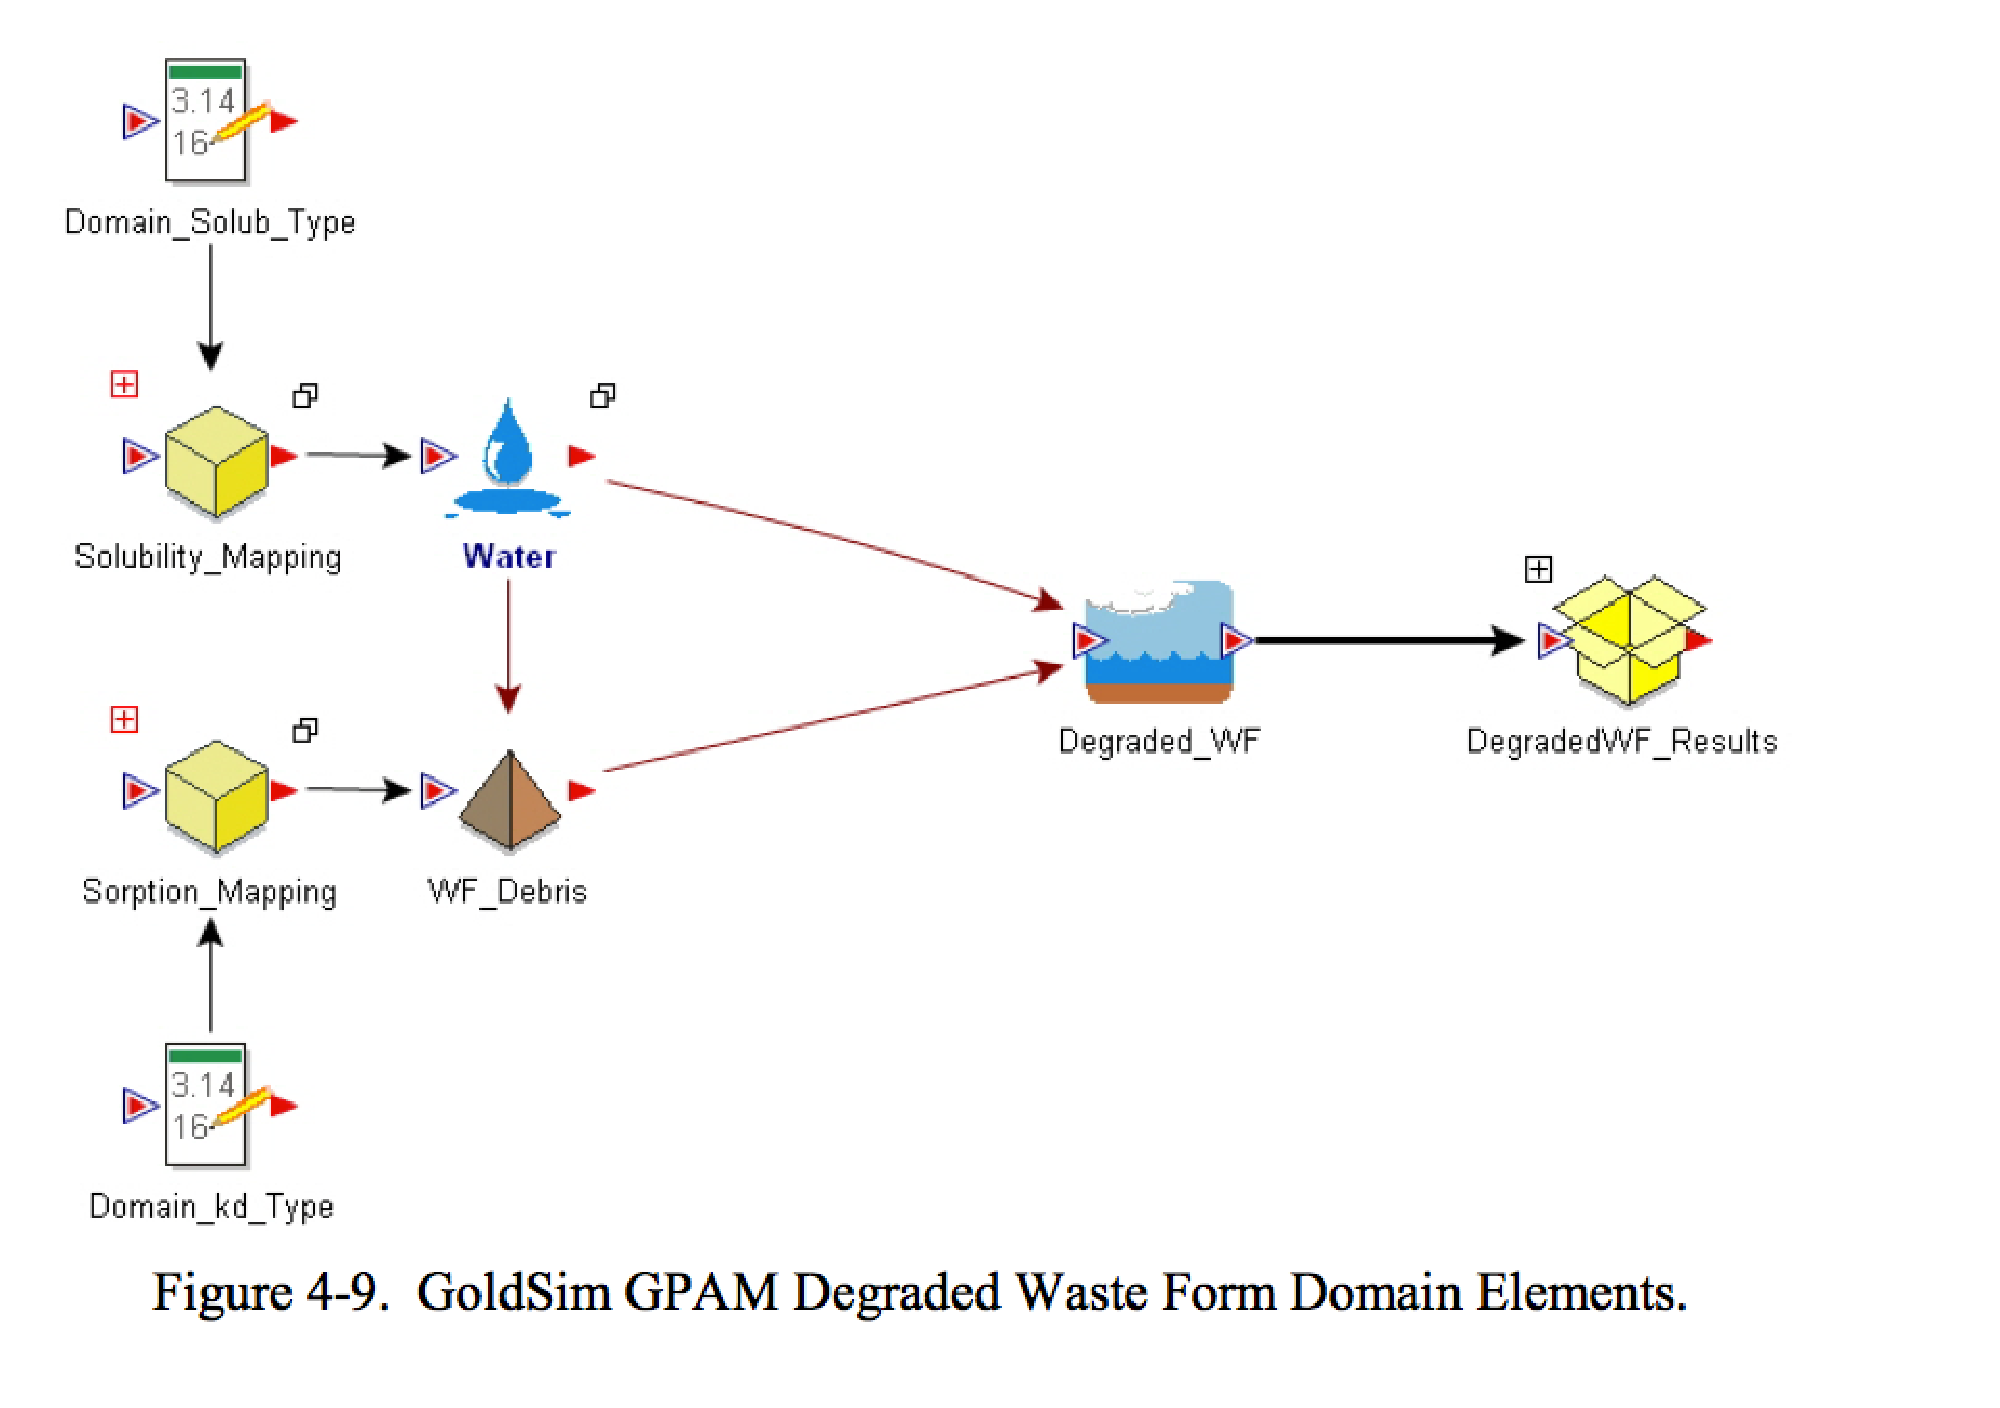
\includegraphics[width=\textwidth]{./images/wf.eps}
      \end{center}
    \end{figure}
  \end{minipage}
  \hspace{0.01cm}\large{$\rightarrow$}\hspace{0.01cm}
  \begin{minipage}{0.45\textwidth}
    \begin{figure}[h!]
      \begin{center}
        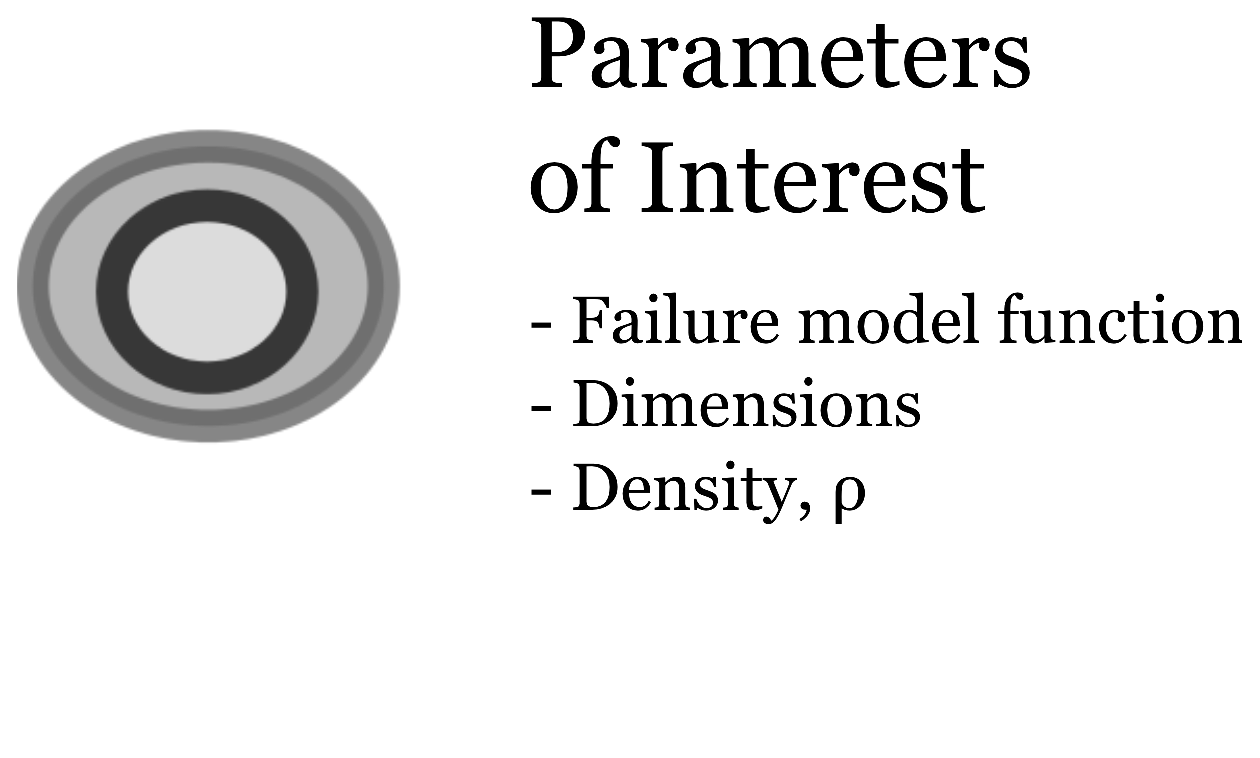
\includegraphics[width=\textwidth]{./images/abstractionWF.eps}
      \end{center}
    \end{figure}
  \end{minipage}
\end{frame}

\begin{frame}[ctb!]
  \frametitle{Base Case : Waste Package Abstraction}
  \begin{minipage}{0.45\textwidth}
    \begin{figure}[h!]
      \begin{center}
        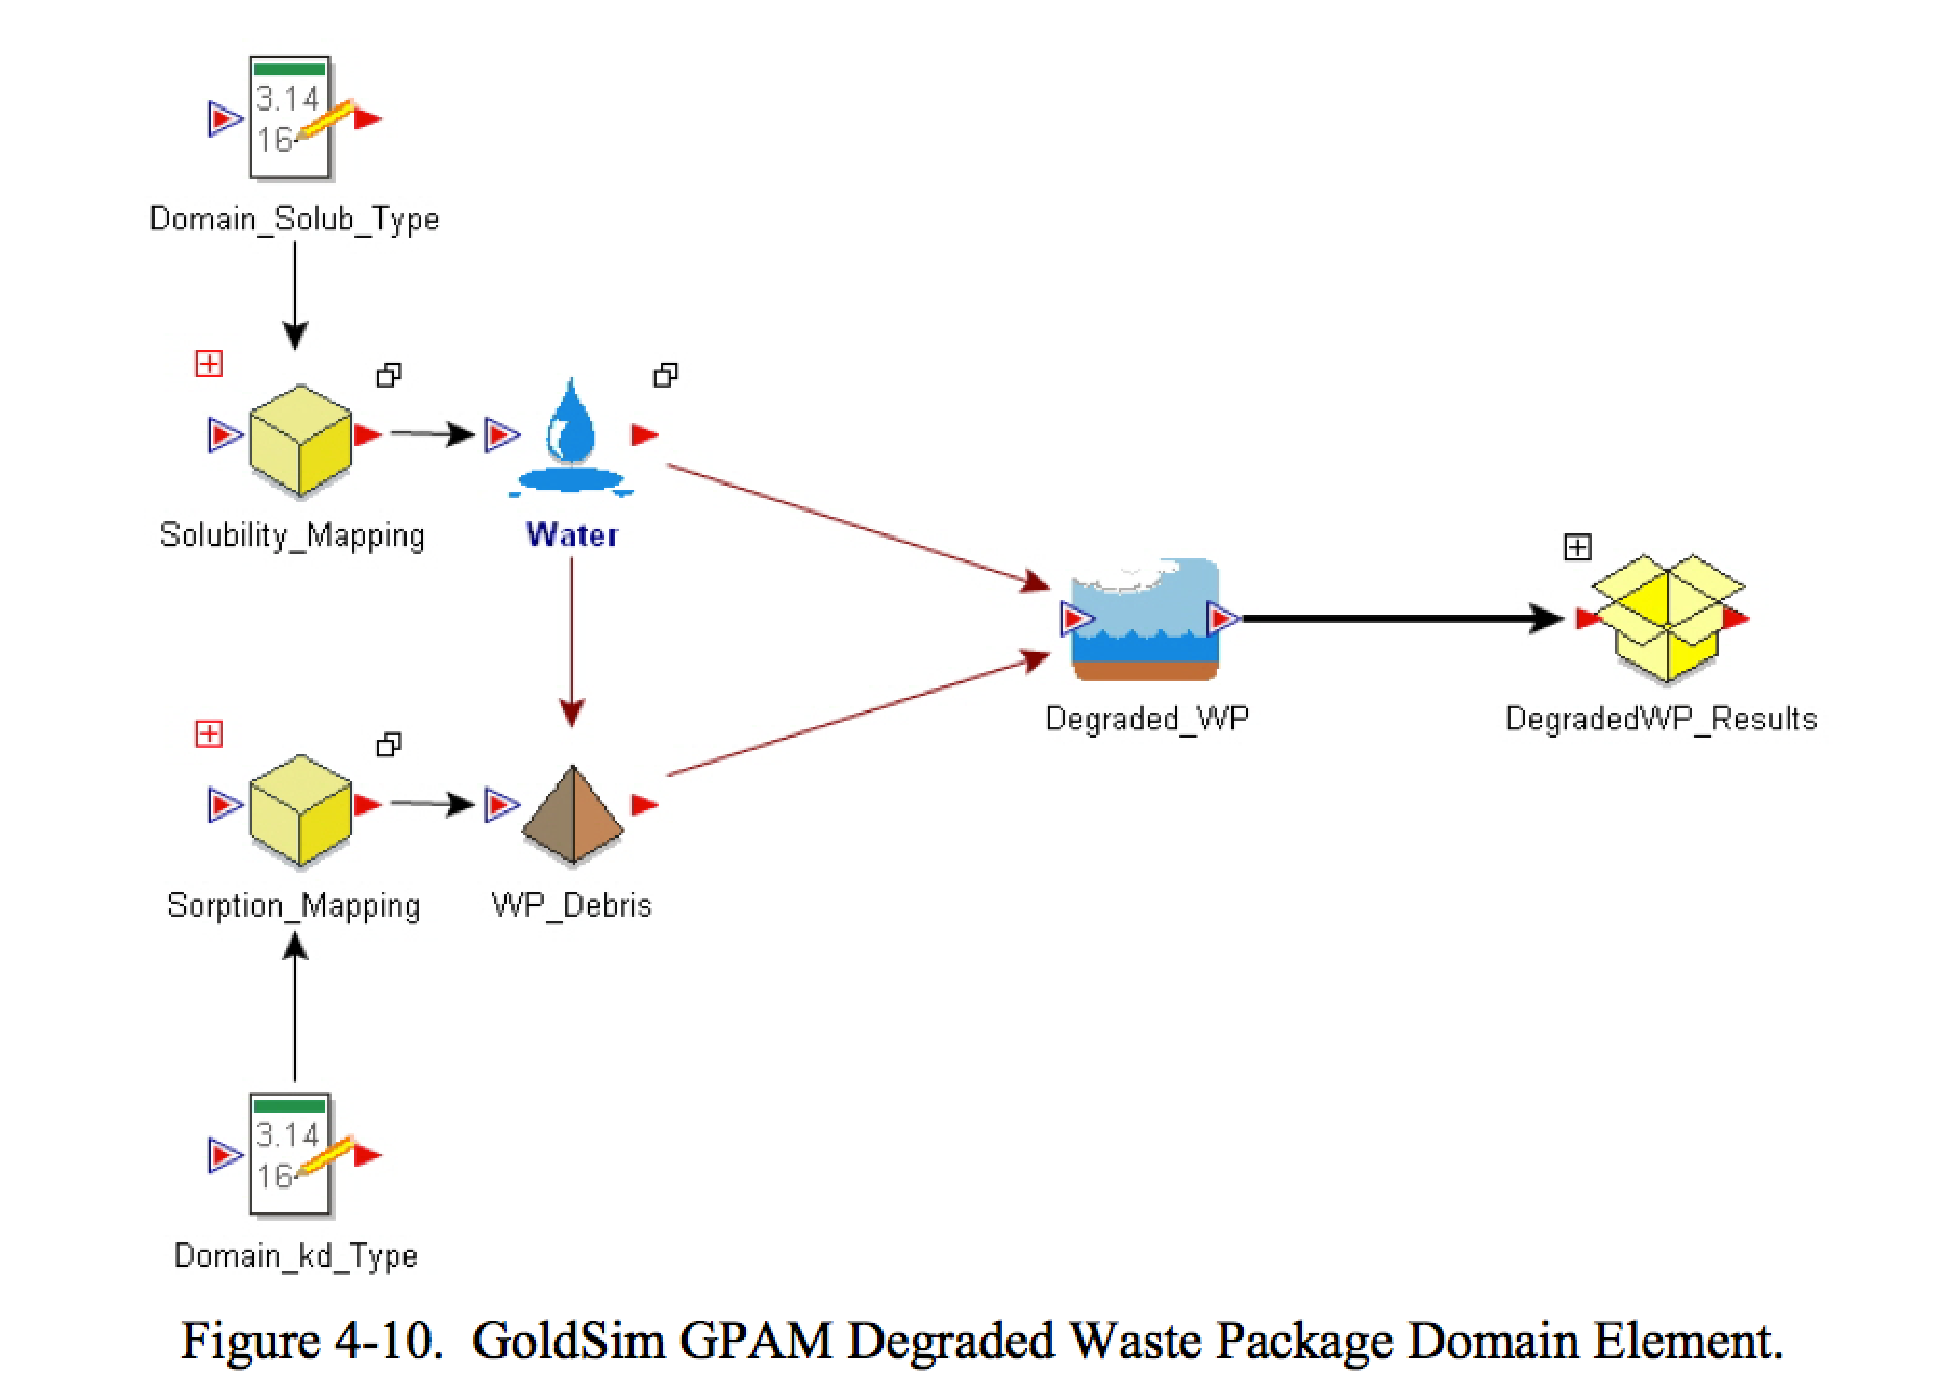
\includegraphics[width=\textwidth]{./images/wp.eps}
      \end{center}
    \end{figure}
  \end{minipage}
  \hspace{0.01cm}\large{$\rightarrow$}\hspace{0.01cm}
  \begin{minipage}{0.45\textwidth}
    \begin{figure}[h!]
      \begin{center}
        \includegraphics[width=\textwidth]{./images/abstractionWP.eps}
      \end{center}
    \end{figure}
  \end{minipage}
\end{frame}

\begin{frame}[ctb!]
  \frametitle{Base Case : Buffer Abstraction}
  \begin{minipage}{0.45\textwidth}
    \begin{figure}[h!]
      \begin{center}
        \includegraphics[width=\textwidth]{./images/buffer.eps}
      \end{center}
    \end{figure}
  \end{minipage}
  \hspace{0.01cm}\large{$\rightarrow$}\hspace{0.01cm}
  \begin{minipage}{0.45\textwidth}
    \begin{figure}[h!]
      \begin{center}
        \includegraphics[width=\textwidth]{./images/abstractionBuffer.eps}
      \end{center}
    \end{figure}
  \end{minipage}
\end{frame}

\begin{frame}[ctb!]
  \frametitle{Base Case : Geology Abstraction}
  \begin{minipage}{0.45\textwidth}
    \begin{figure}[h!]
      \begin{center}
        \includegraphics[width=\textwidth]{./images/rock.eps}
      \end{center}
    \end{figure}
  \end{minipage}
  \hspace{0.01cm}\large{$\rightarrow$}\hspace{0.01cm}
  \begin{minipage}{0.45\textwidth}
    \begin{figure}[h!]
      \begin{center}
        \includegraphics[width=\textwidth]{./images/abstractionRock.eps}
      \end{center}
    \end{figure}
  \end{minipage}
\end{frame}

\begin{frame}[ctb!]
  \frametitle{Base Case : System Level Abstraction}
  \begin{figure}[h!]
      \includegraphics[width=\textwidth]{./images/abstractionSystem.eps}
    \caption{System level abstraction seeks to determine the systems level 
    response to the change in models of subcomponents.}
  \end{figure}
\end{frame}

\subsection{Extensions}


\begin{frame}[ctb!]
  \frametitle{Extensions : Fracturation}
    \begin{minipage}{0.49\textwidth}
      \begin{figure}[h!]
        \includegraphics[width=\textwidth]{./images/fracturesAB.eps}
        \label{fig:fracturesAB}
      \end{figure}
    \end{minipage}
    \hspace{.01cm}
    \begin{minipage}{0.49\textwidth}
      \begin{figure}[h!]
        \includegraphics[width=\textwidth]{./images/fracturesCD.eps}
        \label{fig:fracturesCD}
      \end{figure}
    \end{minipage}

  A dual continuum model will be implemented to more accurately represent 
  fractured host media such as granite \cite{anderson_applied_1992}.
\end{frame}


\begin{frame}[ctb!]
  \frametitle{Extensions : Sorption}
  \begin{figure}[h!]
      \includegraphics[height=.75\textheight]{./images/sorptionKrauskopf.eps}
    \caption{Sorption will be modeled using retardation factors in the mixed 
    cell models \cite{krauskopf_geology_1988}.}
    \label{fig:sorptionKrauskopf}
  \end{figure}
\end{frame}


\begin{frame}[ctb!]
  \frametitle{Extensions : Coalescence}
  Salt and clay exhibit coalescent behavior under heat. This decreases both the 
  buffer volume and the porosity in the near field.
  \begin{figure}[h!]
    \begin{center}
      \includegraphics[width=\textwidth]{./images/saltAlcoveGPAM.eps}
    \end{center}
    \caption{The UFD salt Generic Disposal System Model incorporates salt 
    coalescence by modeling an alcove which decreases in size 
    \cite{clayton_generic_2011}.}
    \label{fig:saltAlcoveGPAM}
  \end{figure}
\end{frame}


\subsection{Summary}


\begin{frame}[ctb!]
  \frametitle{Integrated Used Fuel Disposition and Repository Model}
  %goal
  %method
  %milestones
\end{frame}




%||||---------------
\begin{frame}[allowframebreaks]
  \frametitle{References}
  \bibliographystyle{plain}
  {\footnotesize \bibliography{prelim}}
\end{frame}
%---------------||||




\end{document}

%\begin{frame}[ctb!]
%  \frametitle{Openness}
%  Openness ensures transparency and lowers institutional technical 
%  obstacles to collaboration.
%\end{frame}


